\par En las siguientes figuras se puede ver el algoritmo corrido con distintos valores de $\alpha, \beta$ y $\gamma$.

\par Se observa que mayores valores de $\alpha$ preservan los histogramas originales;
mayores valores de $\beta$ reducen su impacto;
mayores valores de $\gamma$ suavizan el histograma resultante.

\par En particular, con $\alpha = 1$, $H^s = H^0$; con $\beta = 1$, $\forall H^0, H^s = h$\footnote{Con $h$ el $H^t$ resultante de tener un $H^0$ nulo, con $\alpha = 1$.}.

\par Si bien los resultados varían cuantitativamente junto a los parámetros, las únicas diferencias cualitativas se notan para valores altos de $\alpha$ (dentro del intervalo $[0.9, 1]$ en el primer ejemplo).
Variar $\gamma$ afecta la suavidad del histograma pero no parece efectar la suavidad de la imagen\footnote{De hecho el paper sugiere $\gamma = 0$.}.

\begin{figure}[H]
\begin{minipage}[c]{0.48\linewidth}
  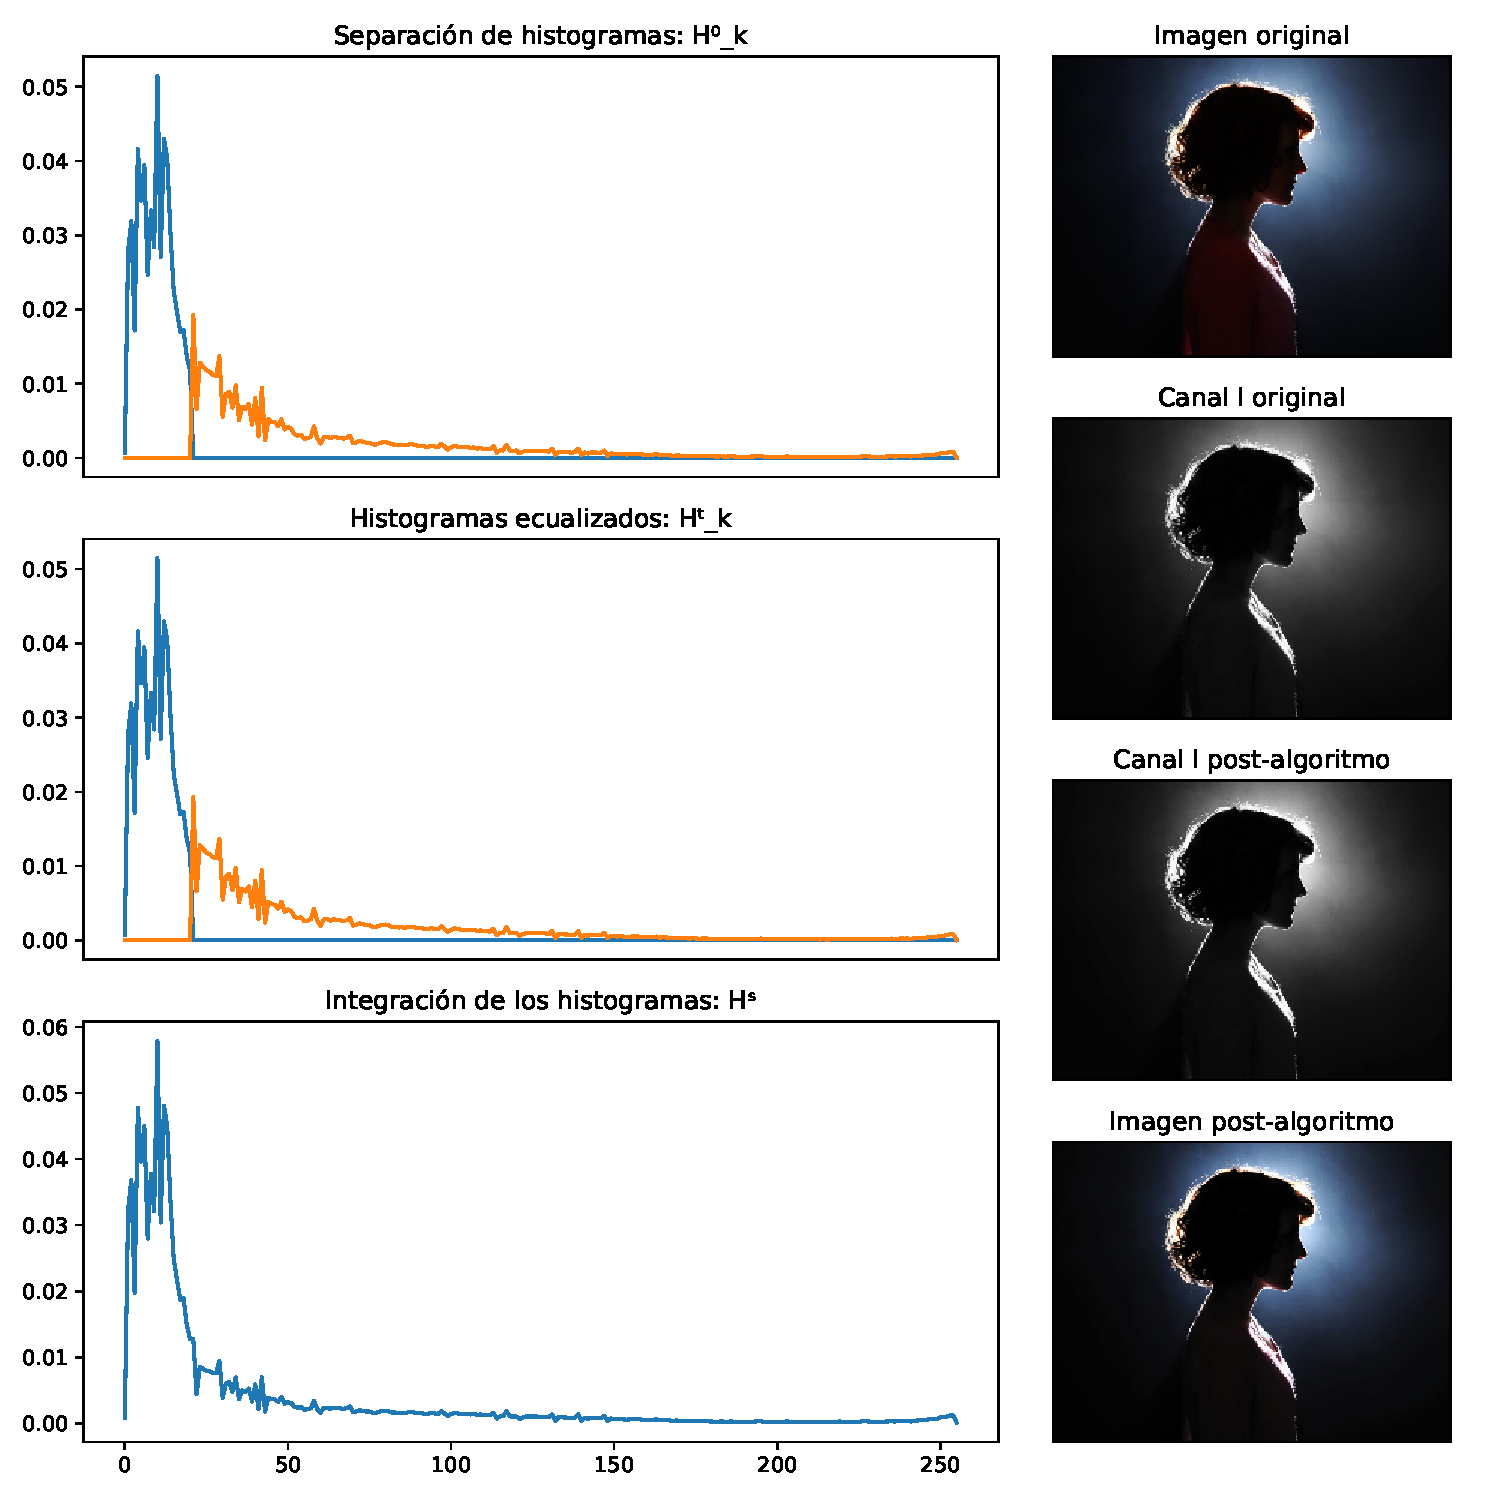
\includegraphics[height=9cm]{imgs/wom-1-0-0.pdf}
  \caption{$\alpha = 1, \beta = 0, \gamma = 0$}
\end{minipage}
\hfill
\begin{minipage}[c]{0.48\linewidth}
  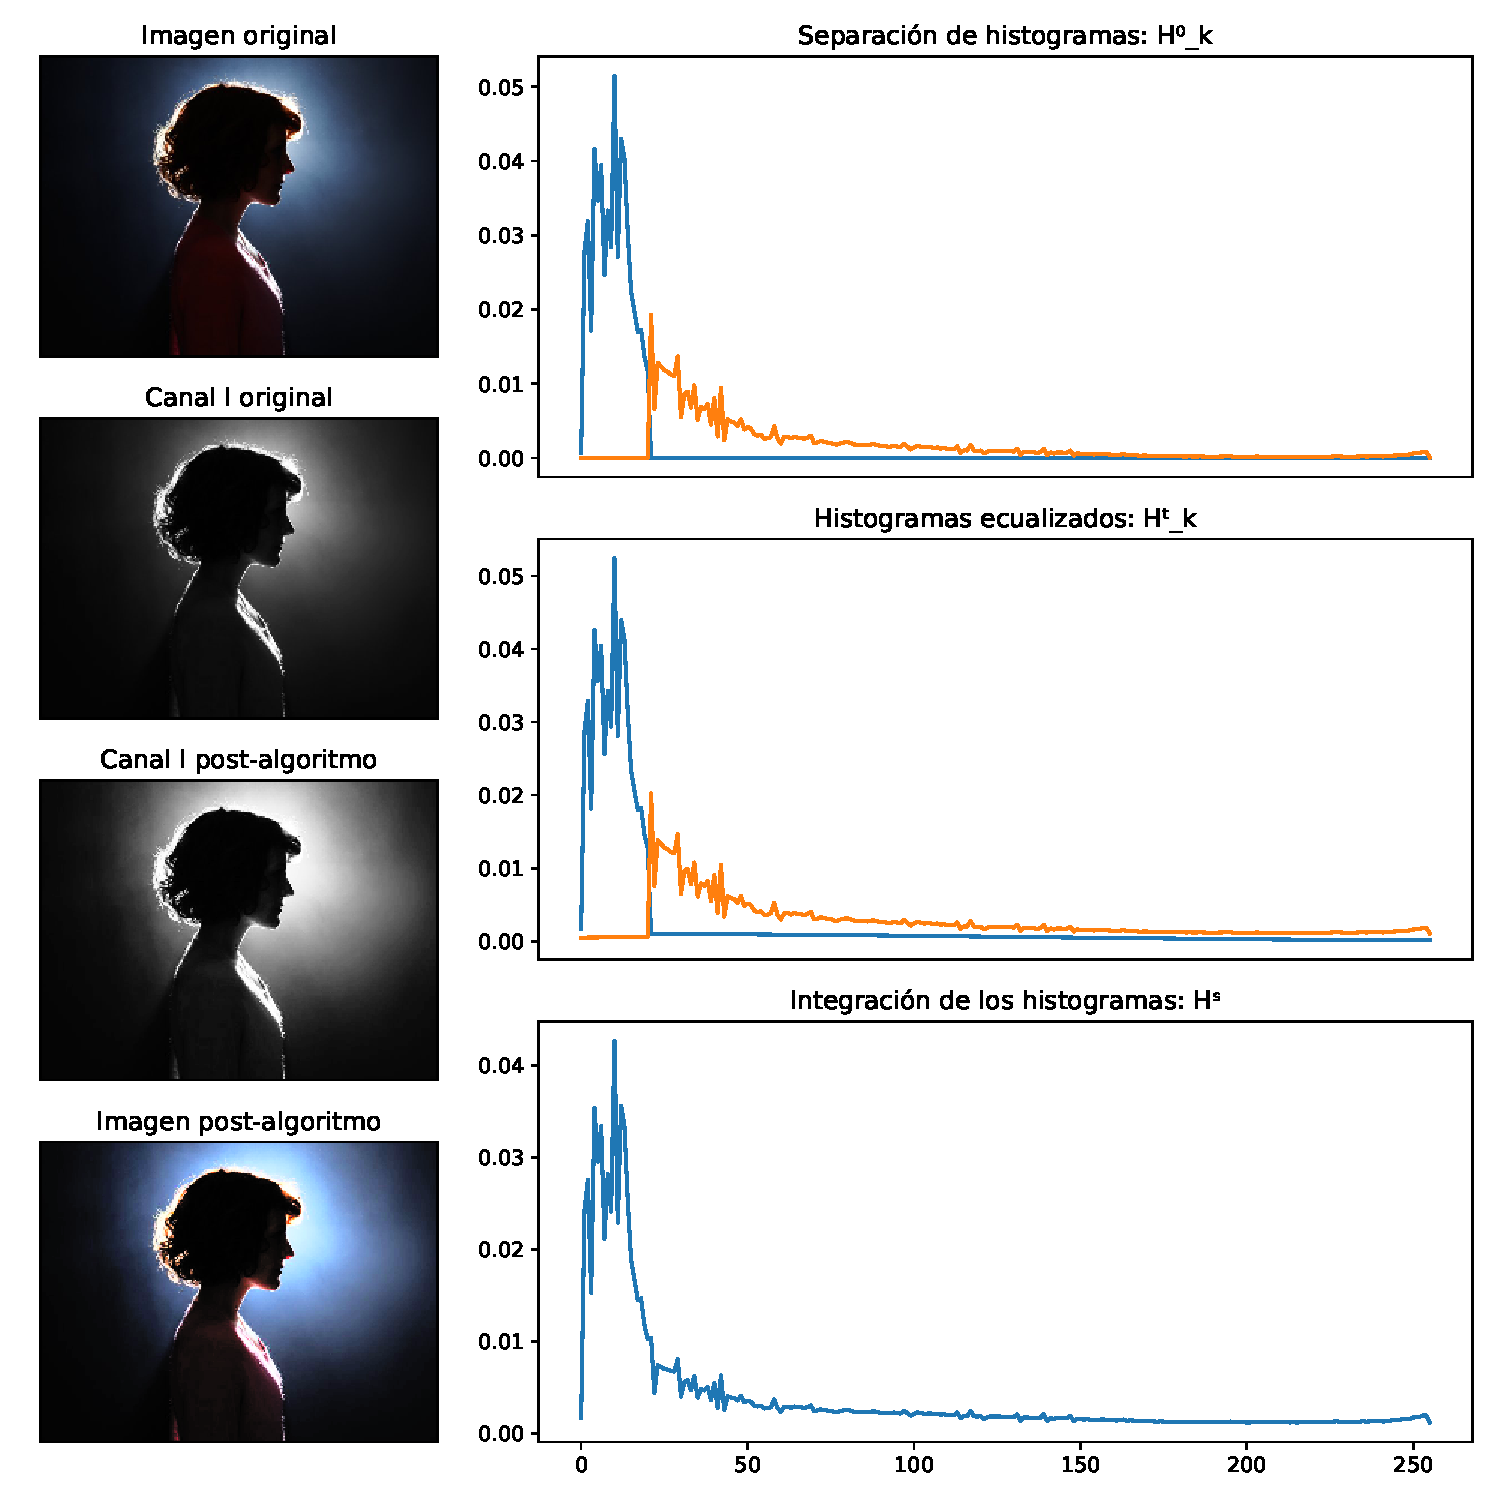
\includegraphics[height=9cm]{imgs/wom-999-001-0.pdf}
  \caption{$\alpha = 0.999, \beta = 0.001, \gamma = 0$}
\end{minipage}%
\end{figure}

\begin{figure}[H]
\begin{minipage}[c]{0.48\linewidth}
  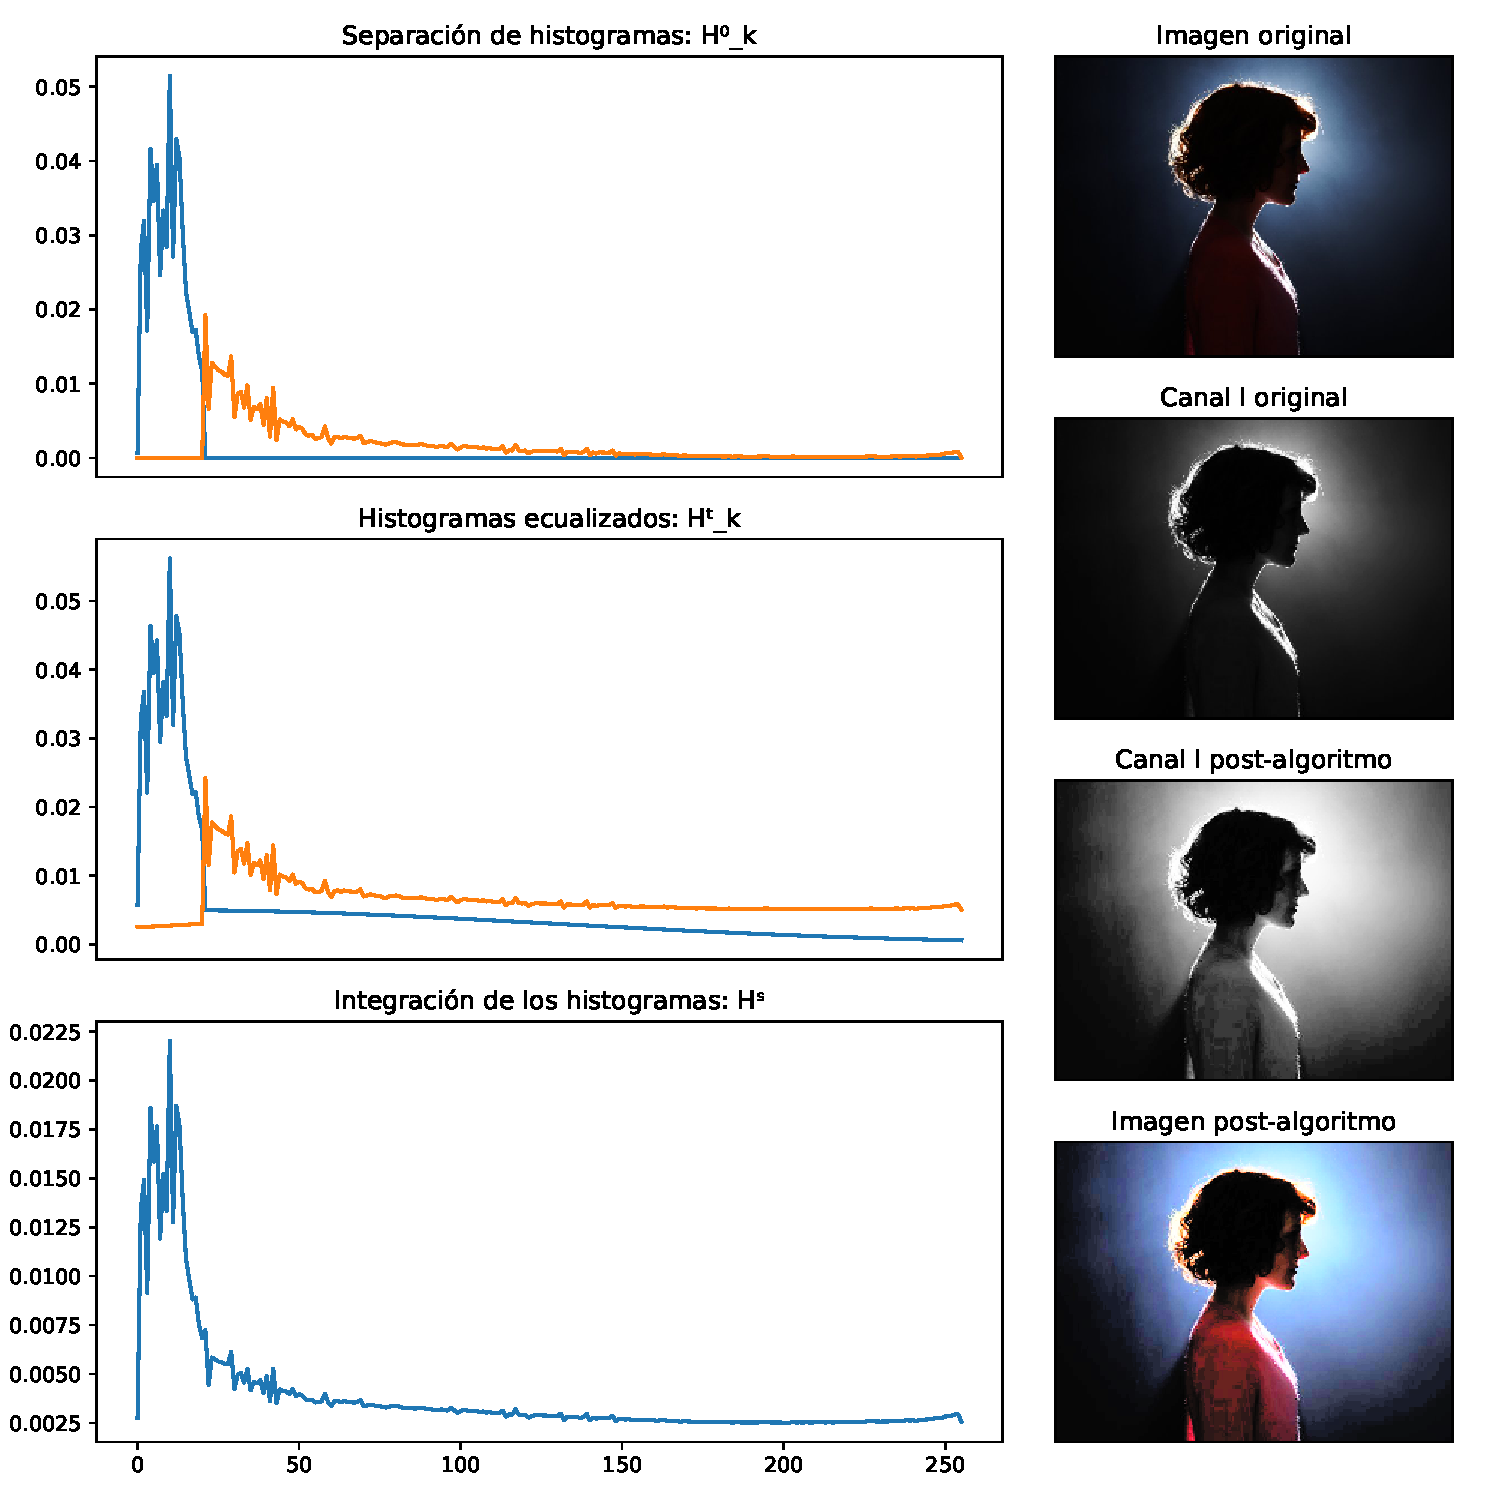
\includegraphics[height=9cm]{imgs/wom-995-005-0.pdf}
  \caption{$\alpha = 0.995, \beta = 0.005, \gamma = 0$}
\end{minipage}
\hfill
\begin{minipage}[c]{0.48\linewidth}
  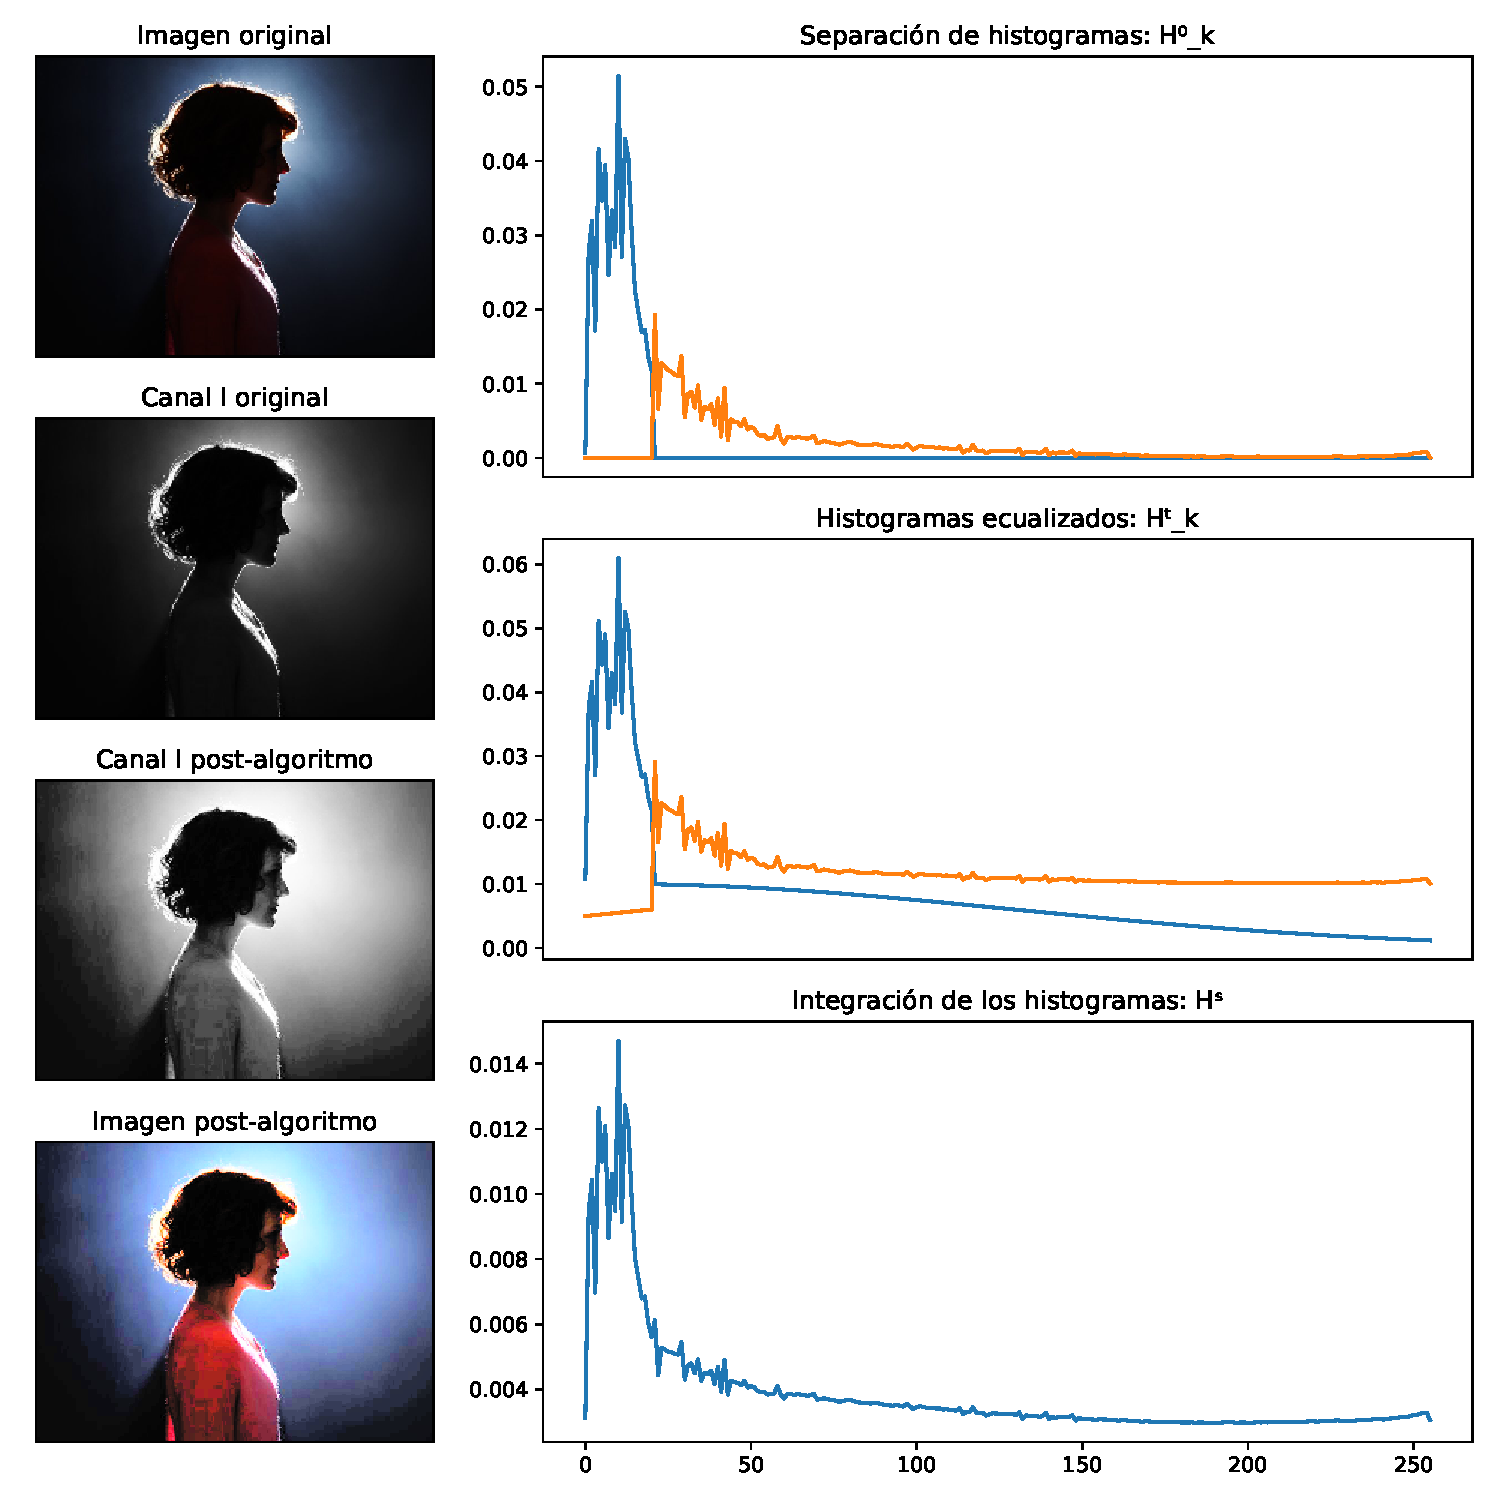
\includegraphics[height=9cm]{imgs/wom-99-01-0.pdf}
  \caption{$\alpha = 0.99, \beta = 0.01, \gamma = 0$}
\end{minipage}%
\end{figure}

\begin{figure}[H]
\begin{minipage}[c]{0.48\linewidth}
  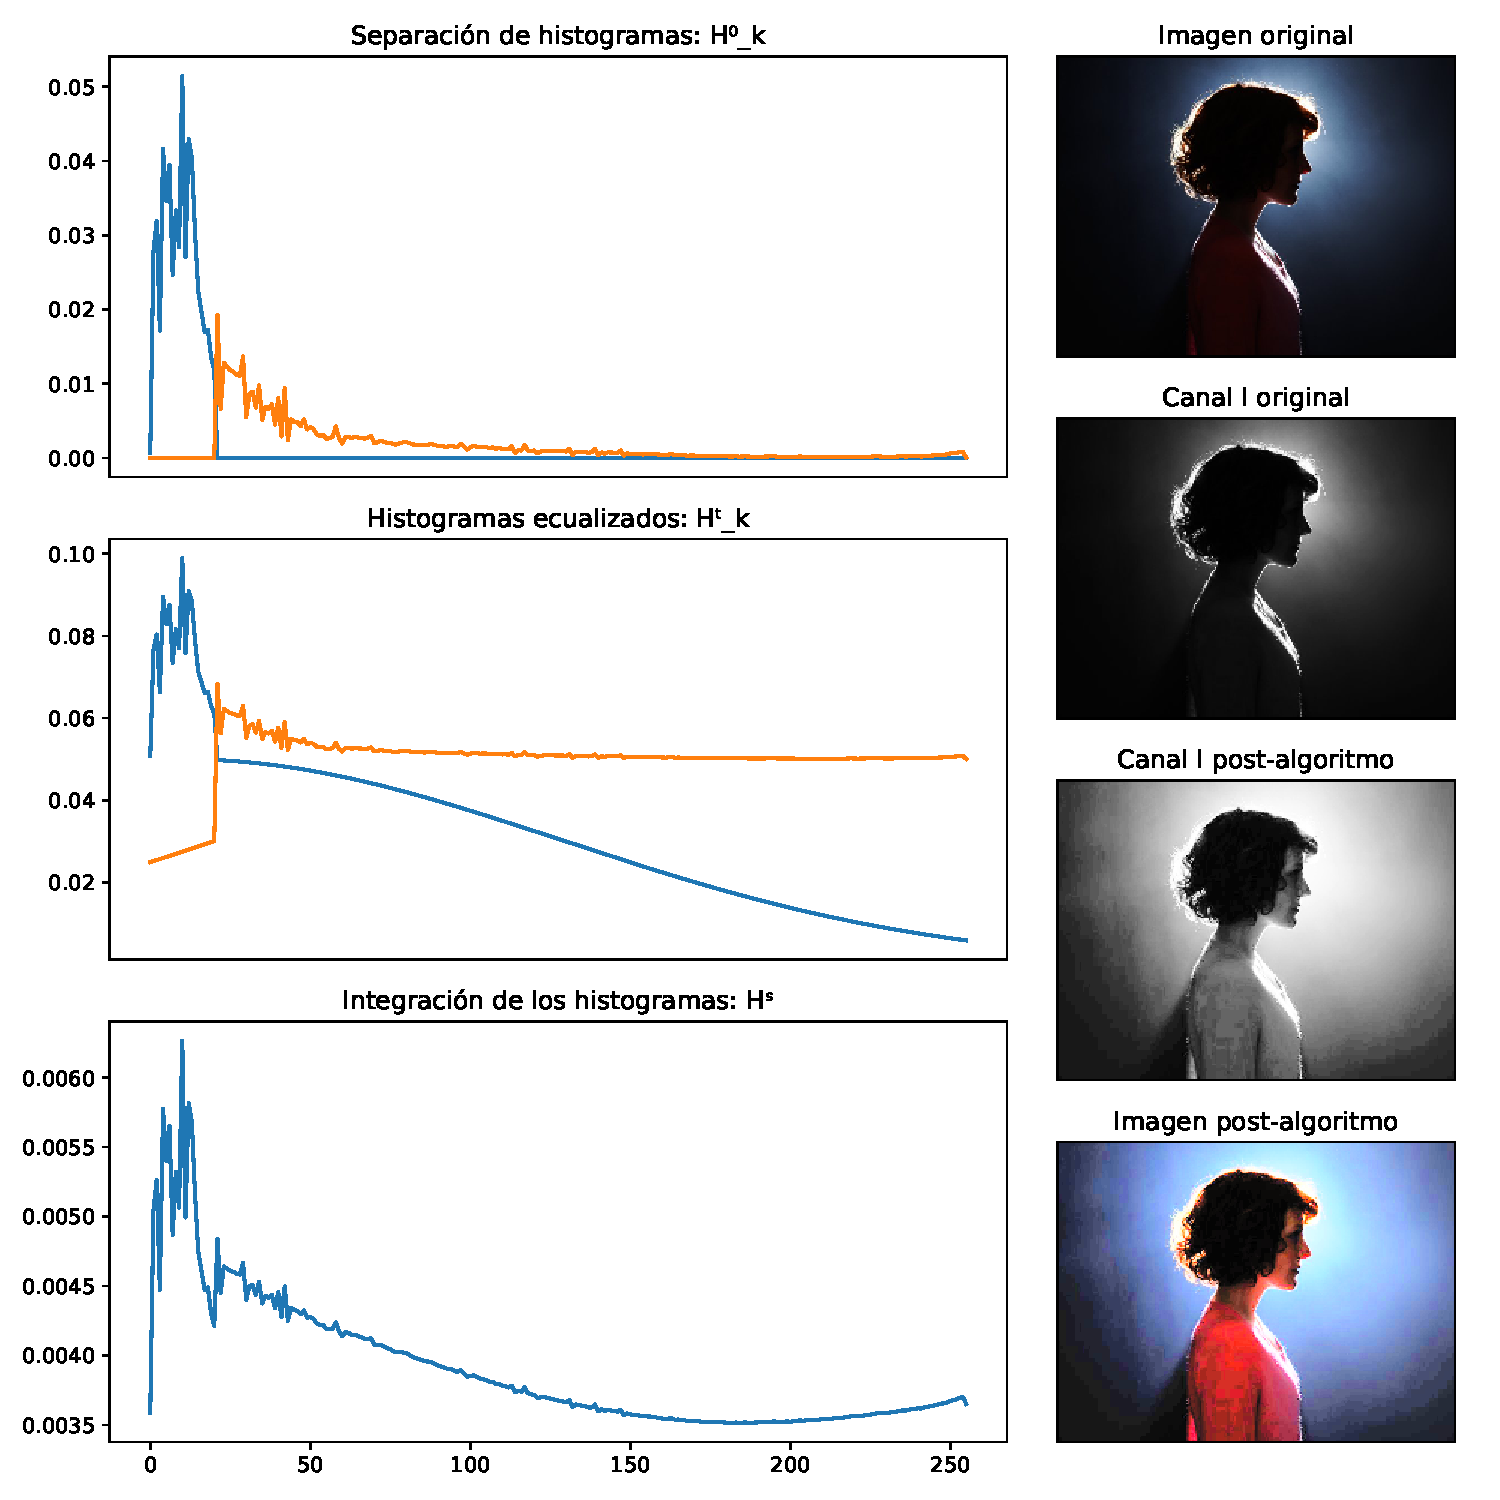
\includegraphics[height=9cm]{imgs/wom-95-05-0.pdf}
  \caption{$\alpha = 0.95, \beta = 0.05, \gamma = 0$}
\end{minipage}
\hfill
\begin{minipage}[c]{0.48\linewidth}
  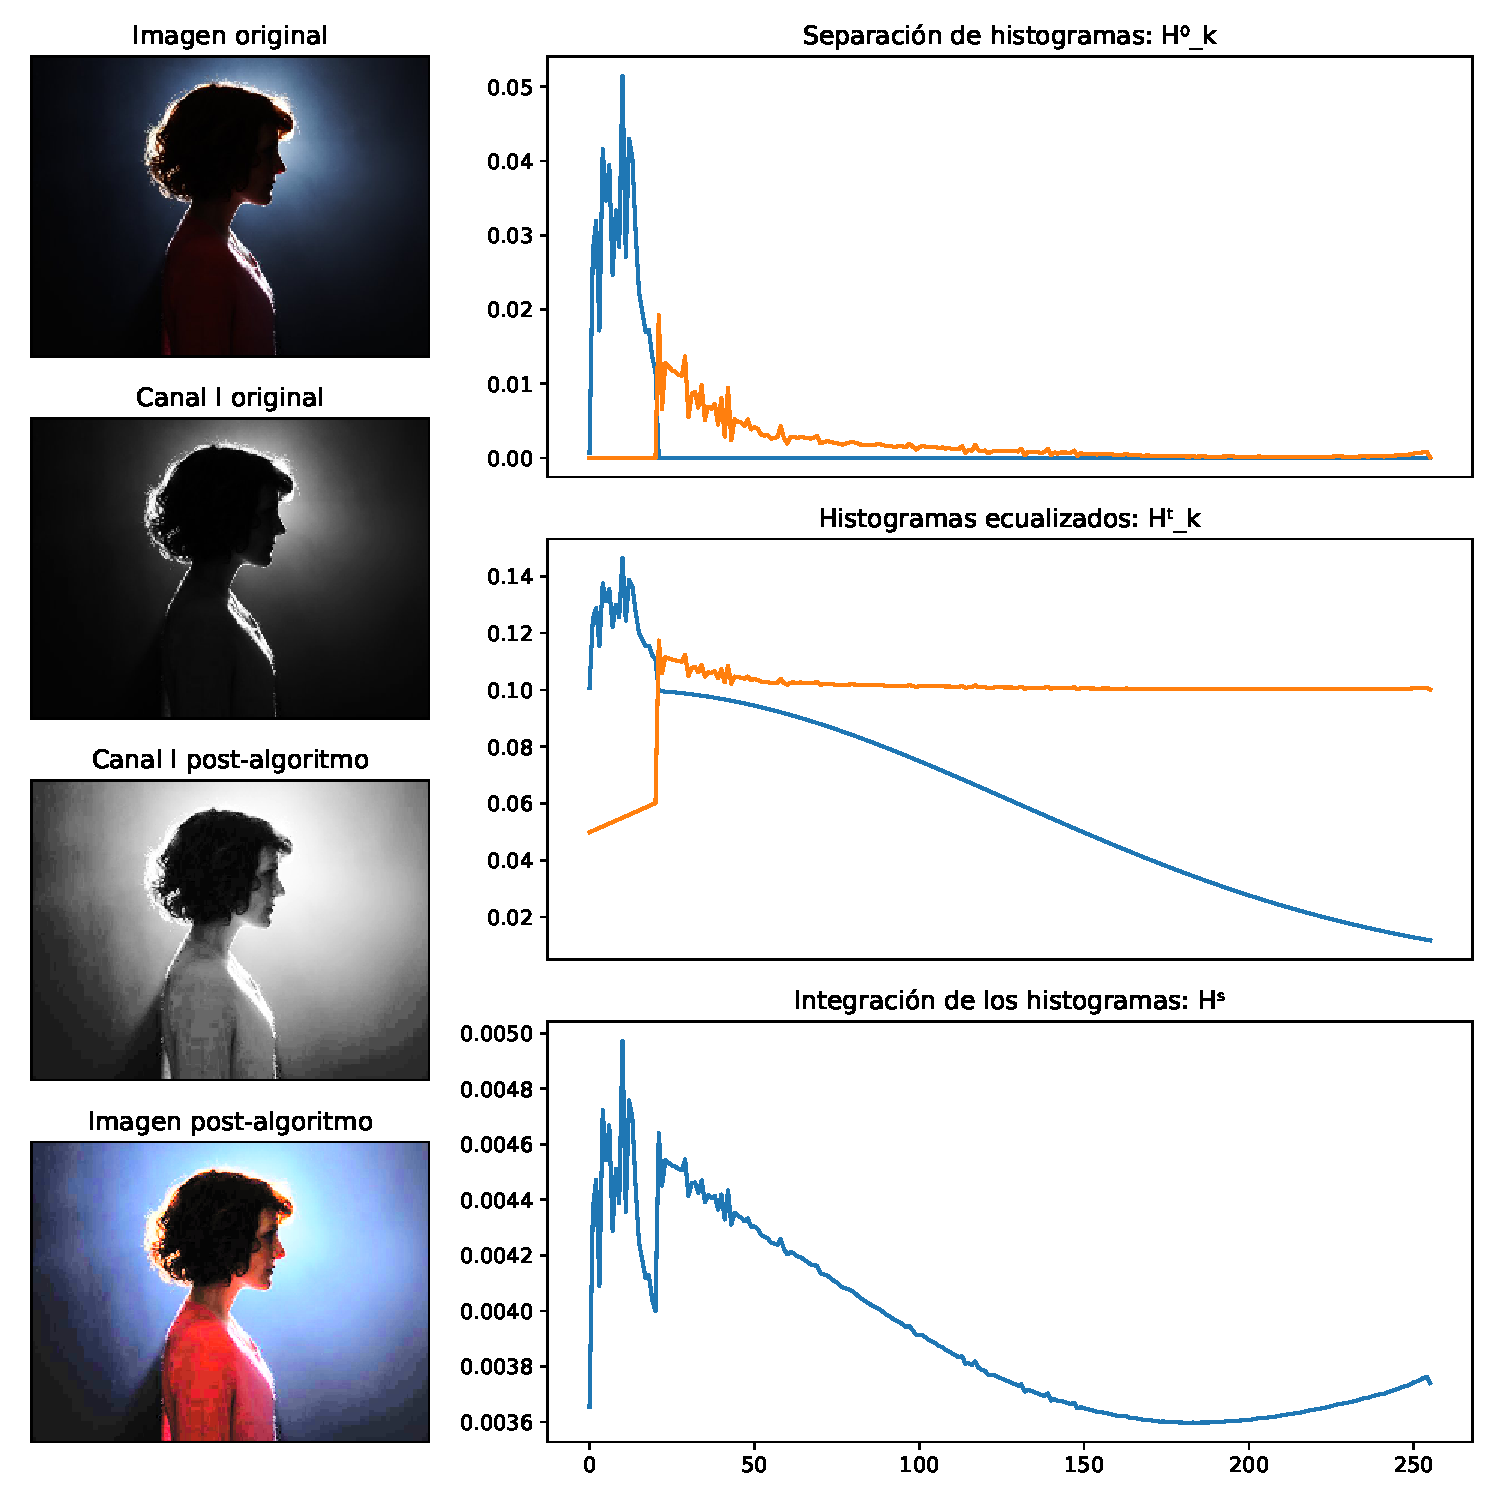
\includegraphics[height=9cm]{imgs/wom-9-1-0.pdf}
  \caption{$\alpha = 0.9, \beta = 0.1, \gamma = 0$}
\end{minipage}%
\end{figure}

\begin{figure}[H]
\begin{minipage}[c]{0.48\linewidth}
  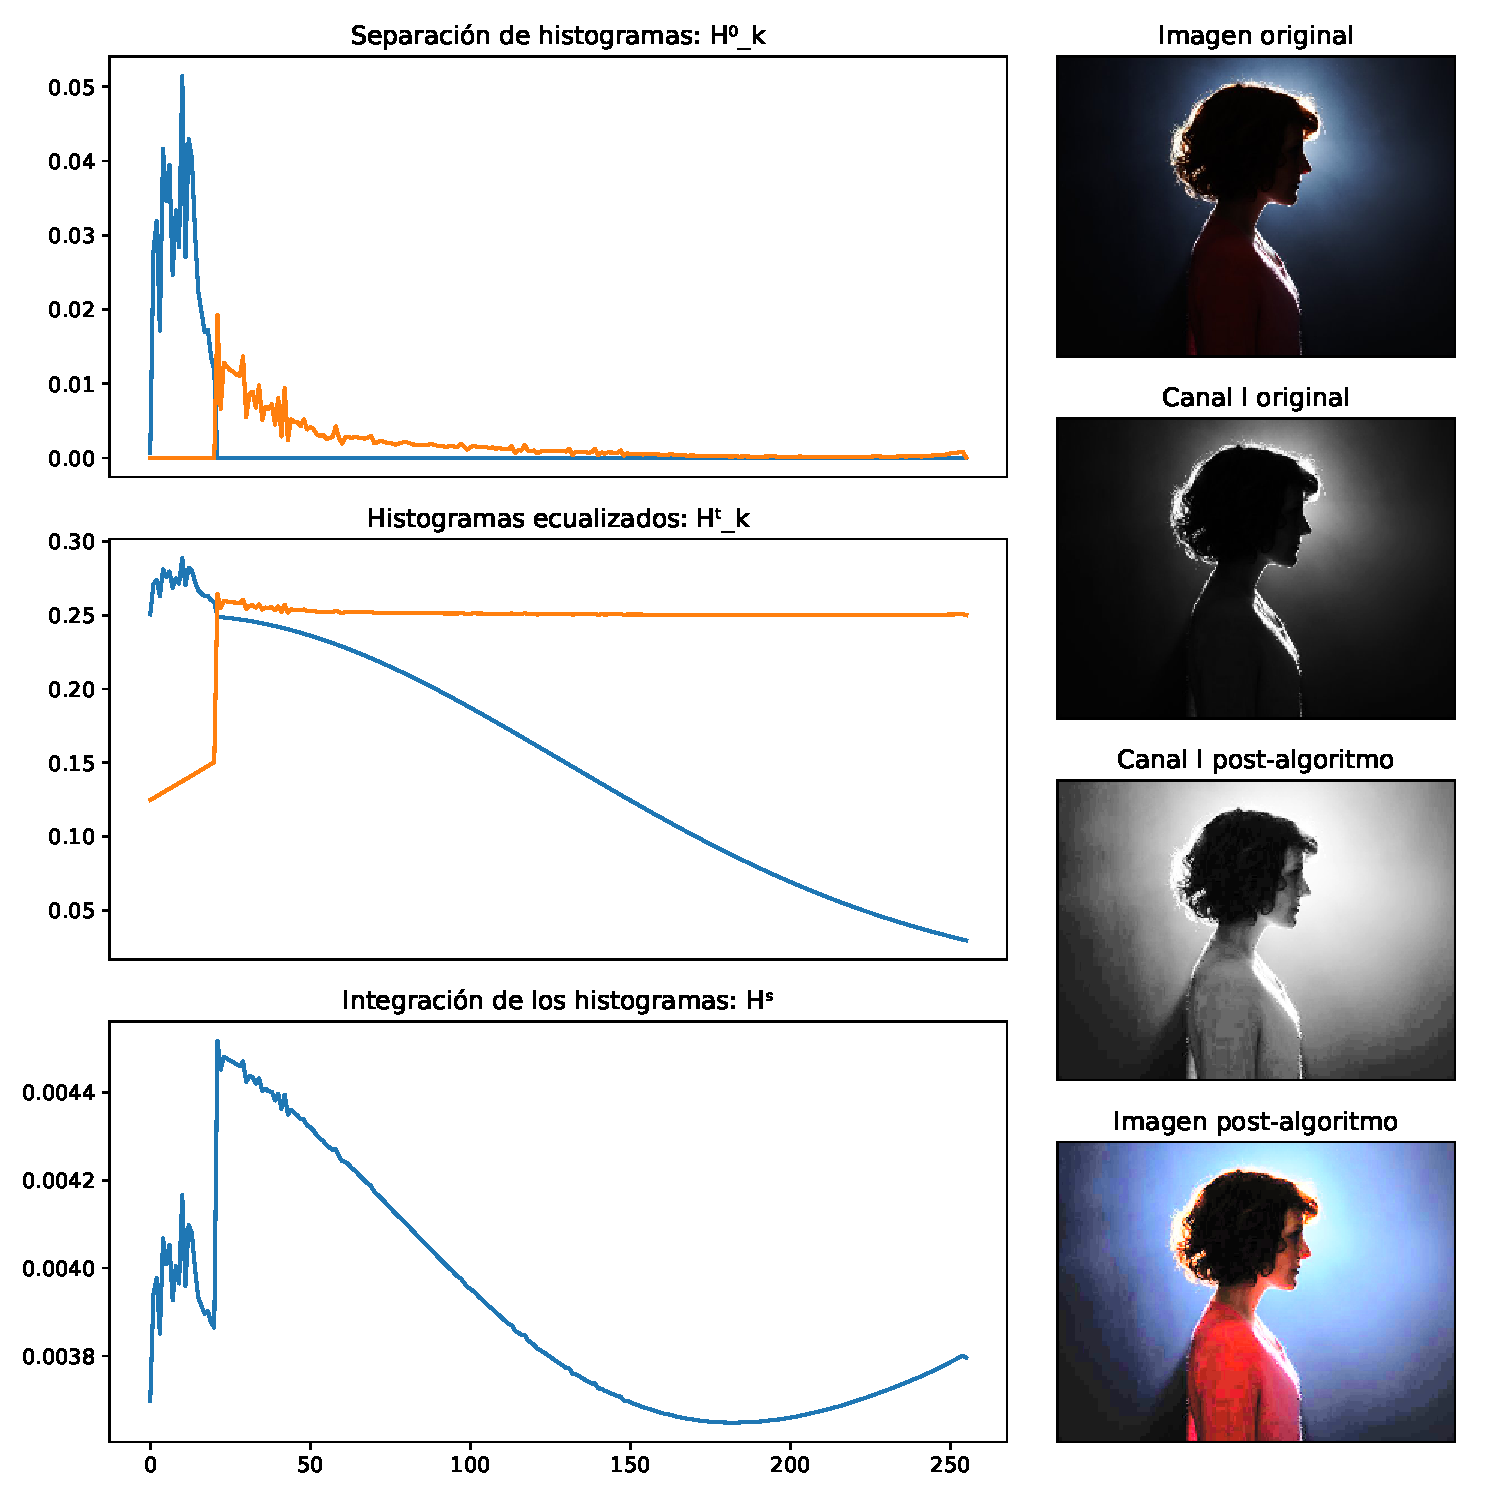
\includegraphics[height=9cm]{imgs/wom-75-25-0.pdf}
  \caption{$\alpha = 0.75, \beta = 0.25, \gamma = 0$}
\end{minipage}
\hfill
\begin{minipage}[c]{0.48\linewidth}
  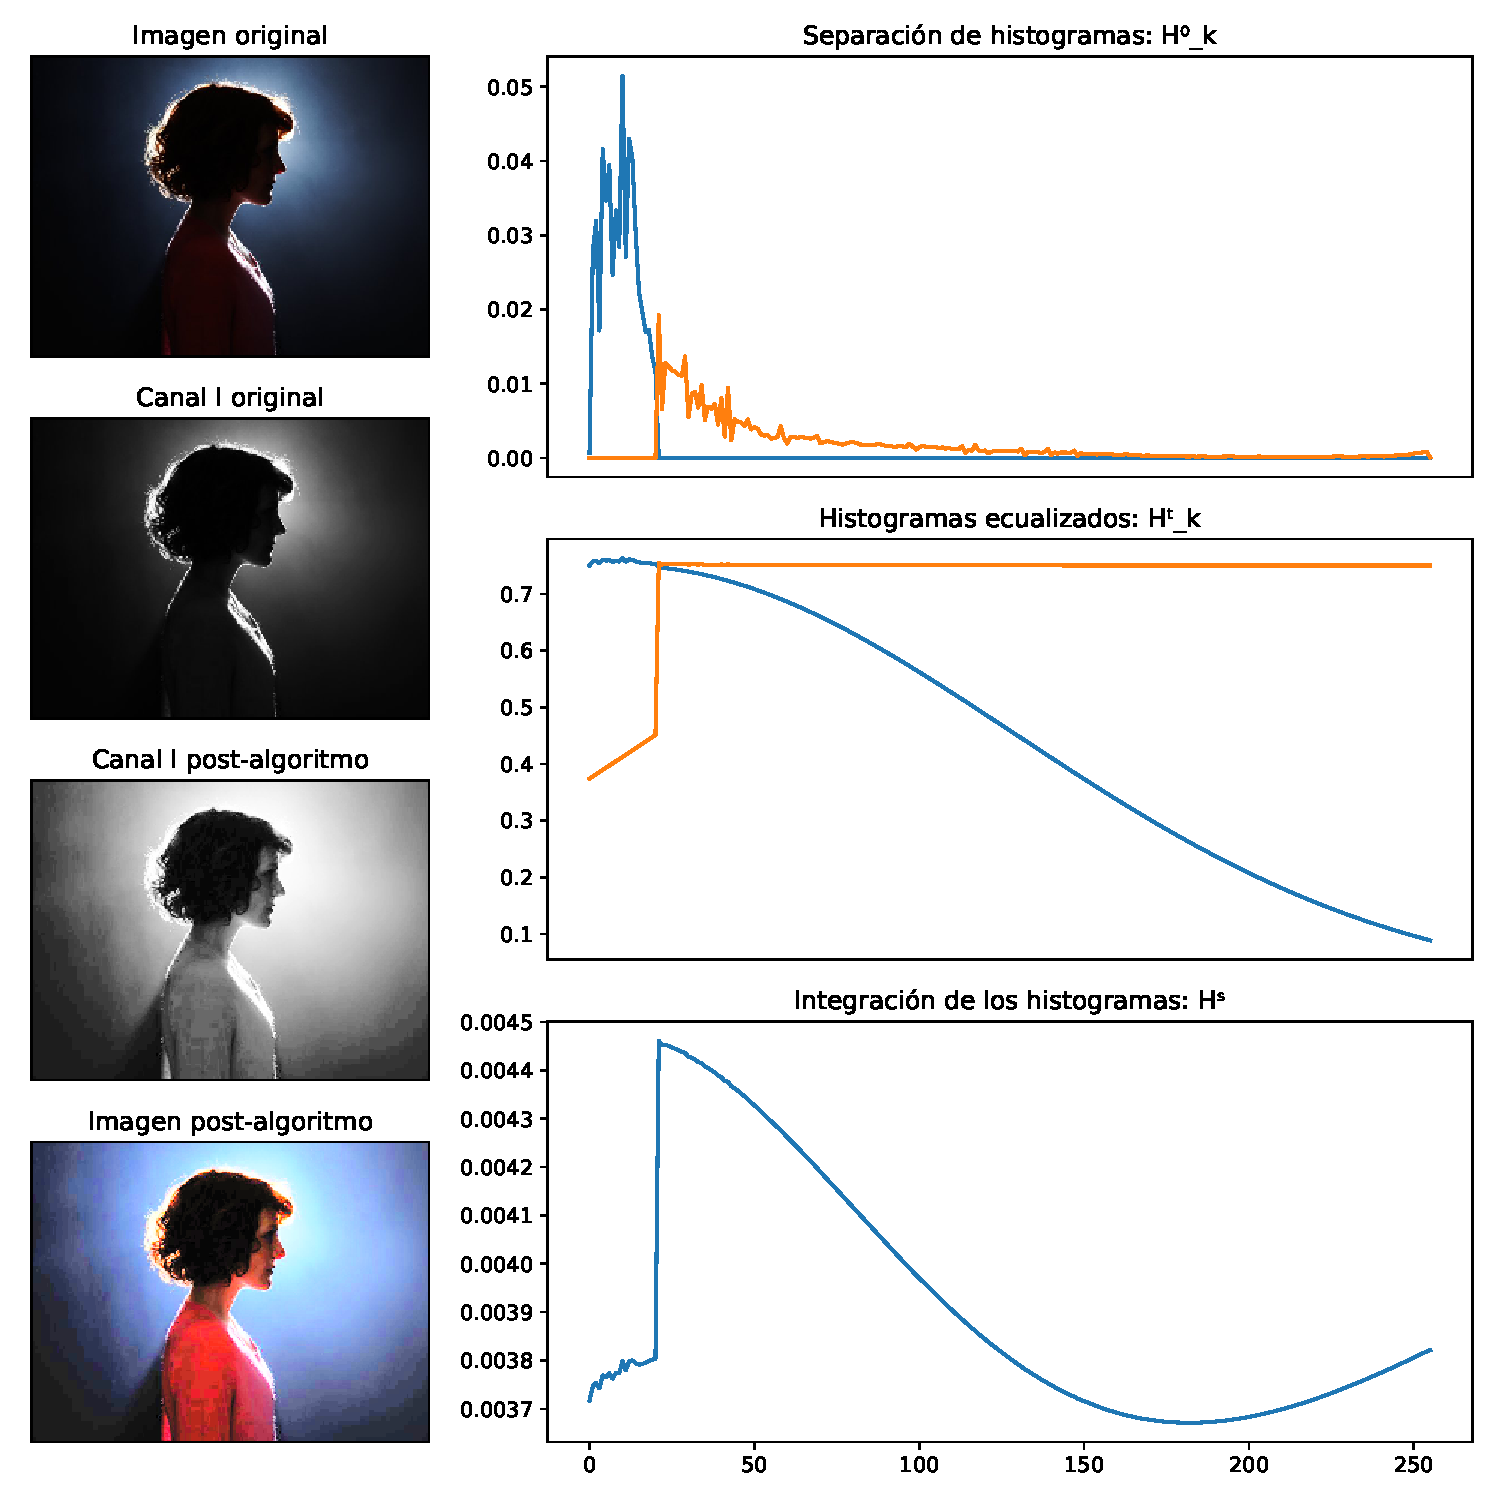
\includegraphics[height=9cm]{imgs/wom-25-75-0.pdf}
  \caption{$\alpha = 0.25, \beta = 0.75, \gamma = 0$}
\end{minipage}%
\end{figure}

\begin{figure}[H]
\begin{minipage}[c]{0.48\linewidth}
  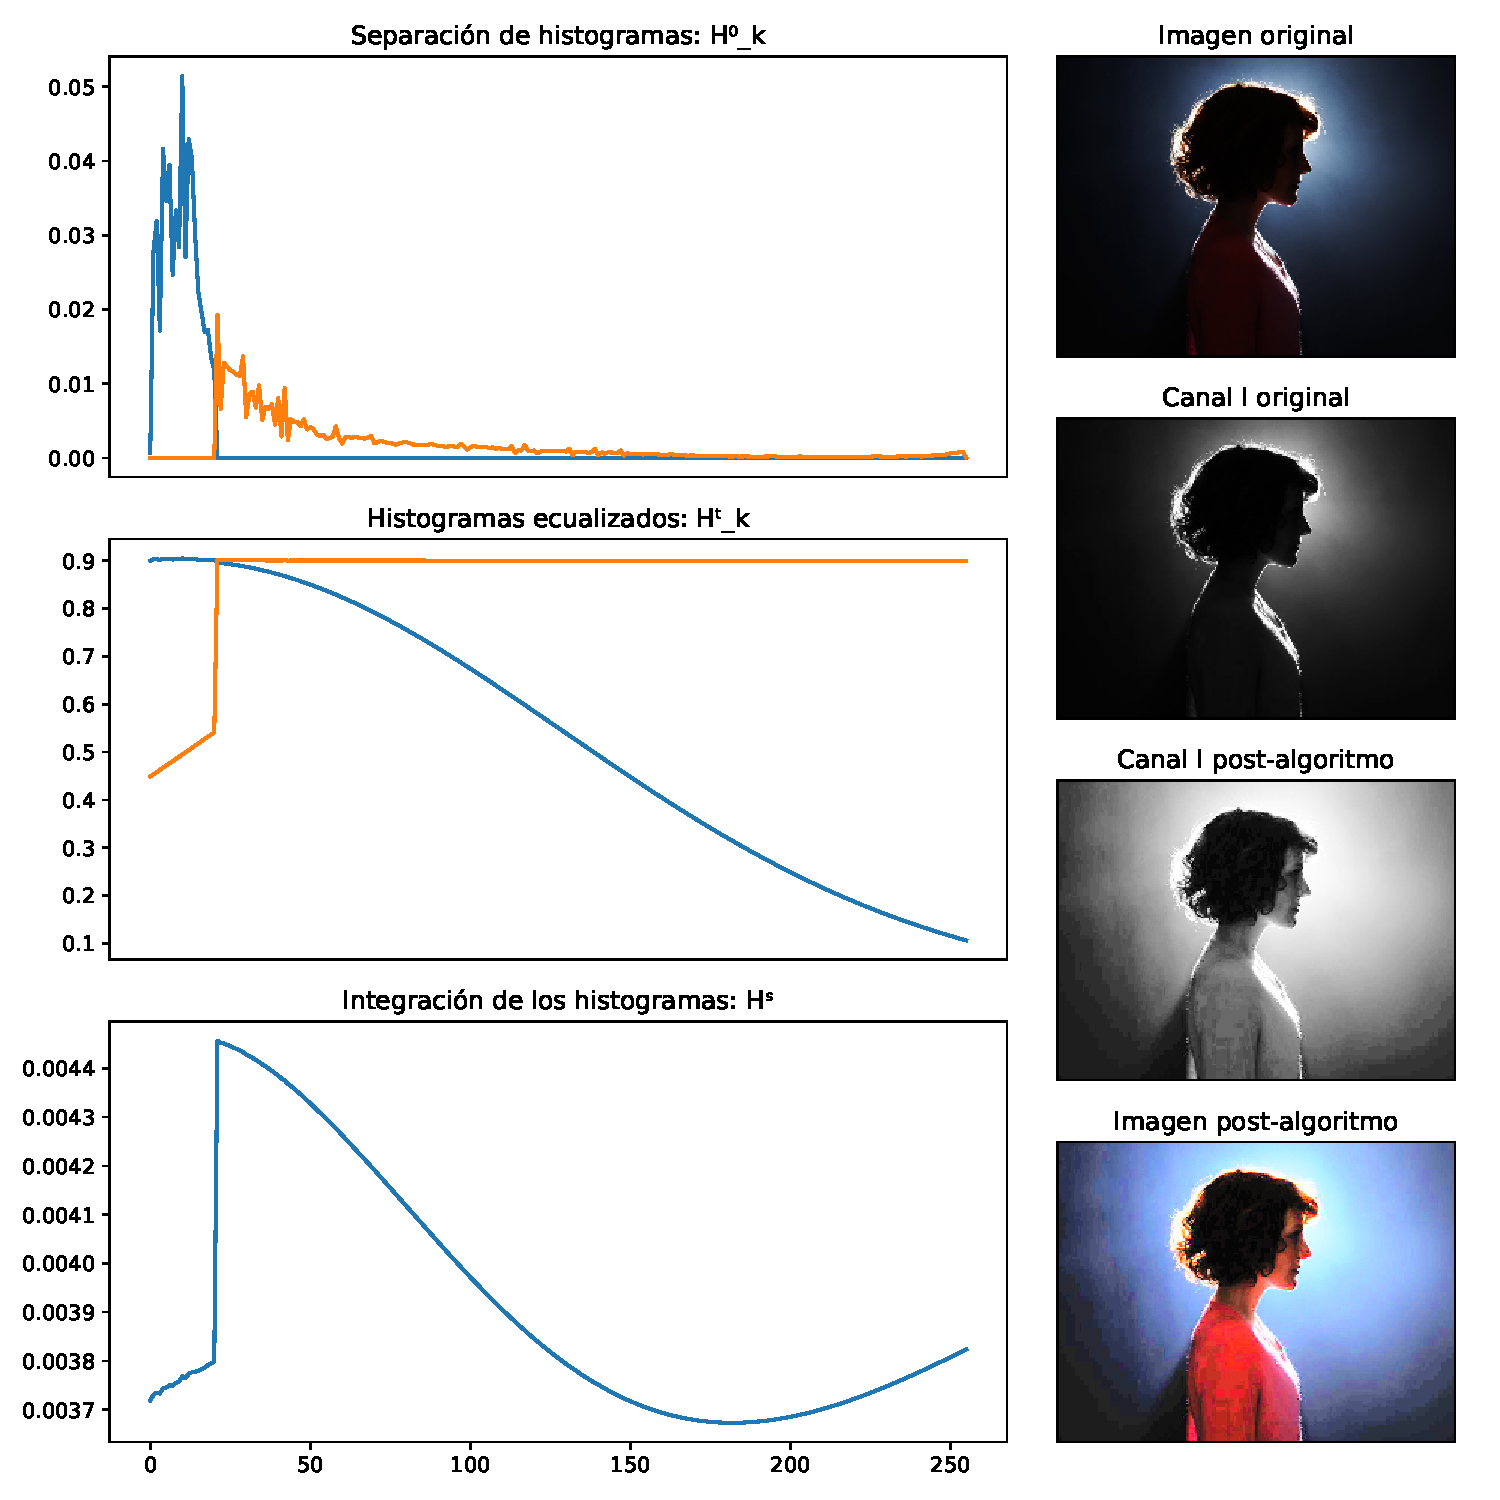
\includegraphics[height=9cm]{imgs/wom-1-9-0.pdf}
  \caption{$\alpha = 0.1, \beta = 0.9, \gamma = 0$}
\end{minipage}
\hfill
\begin{minipage}[c]{0.48\linewidth}
  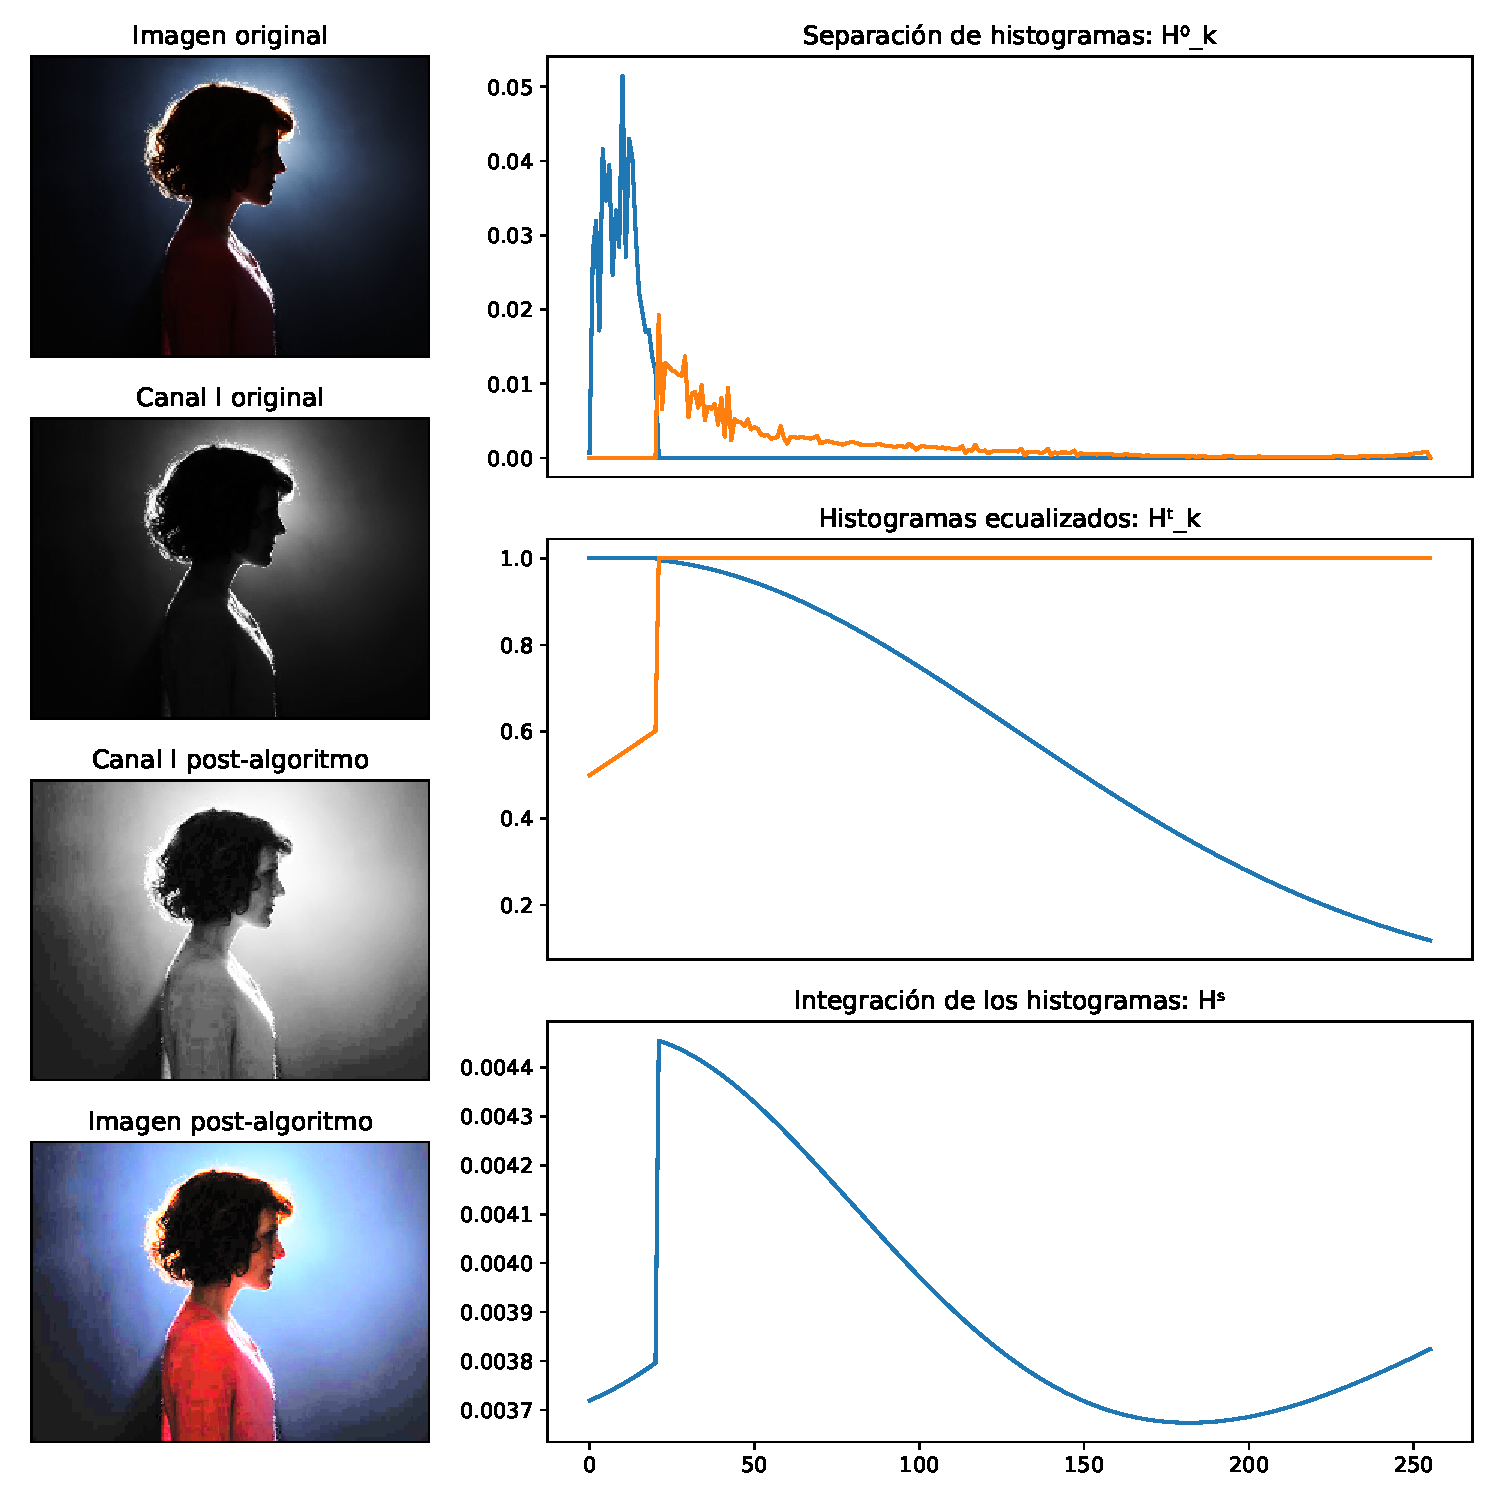
\includegraphics[height=9cm]{imgs/wom-0-1-0.pdf}
  \caption{$\alpha = 0, \beta = 1, \gamma = 0$}
\end{minipage}%
\end{figure}

\begin{figure}[H]
\begin{minipage}[c]{0.48\linewidth}
  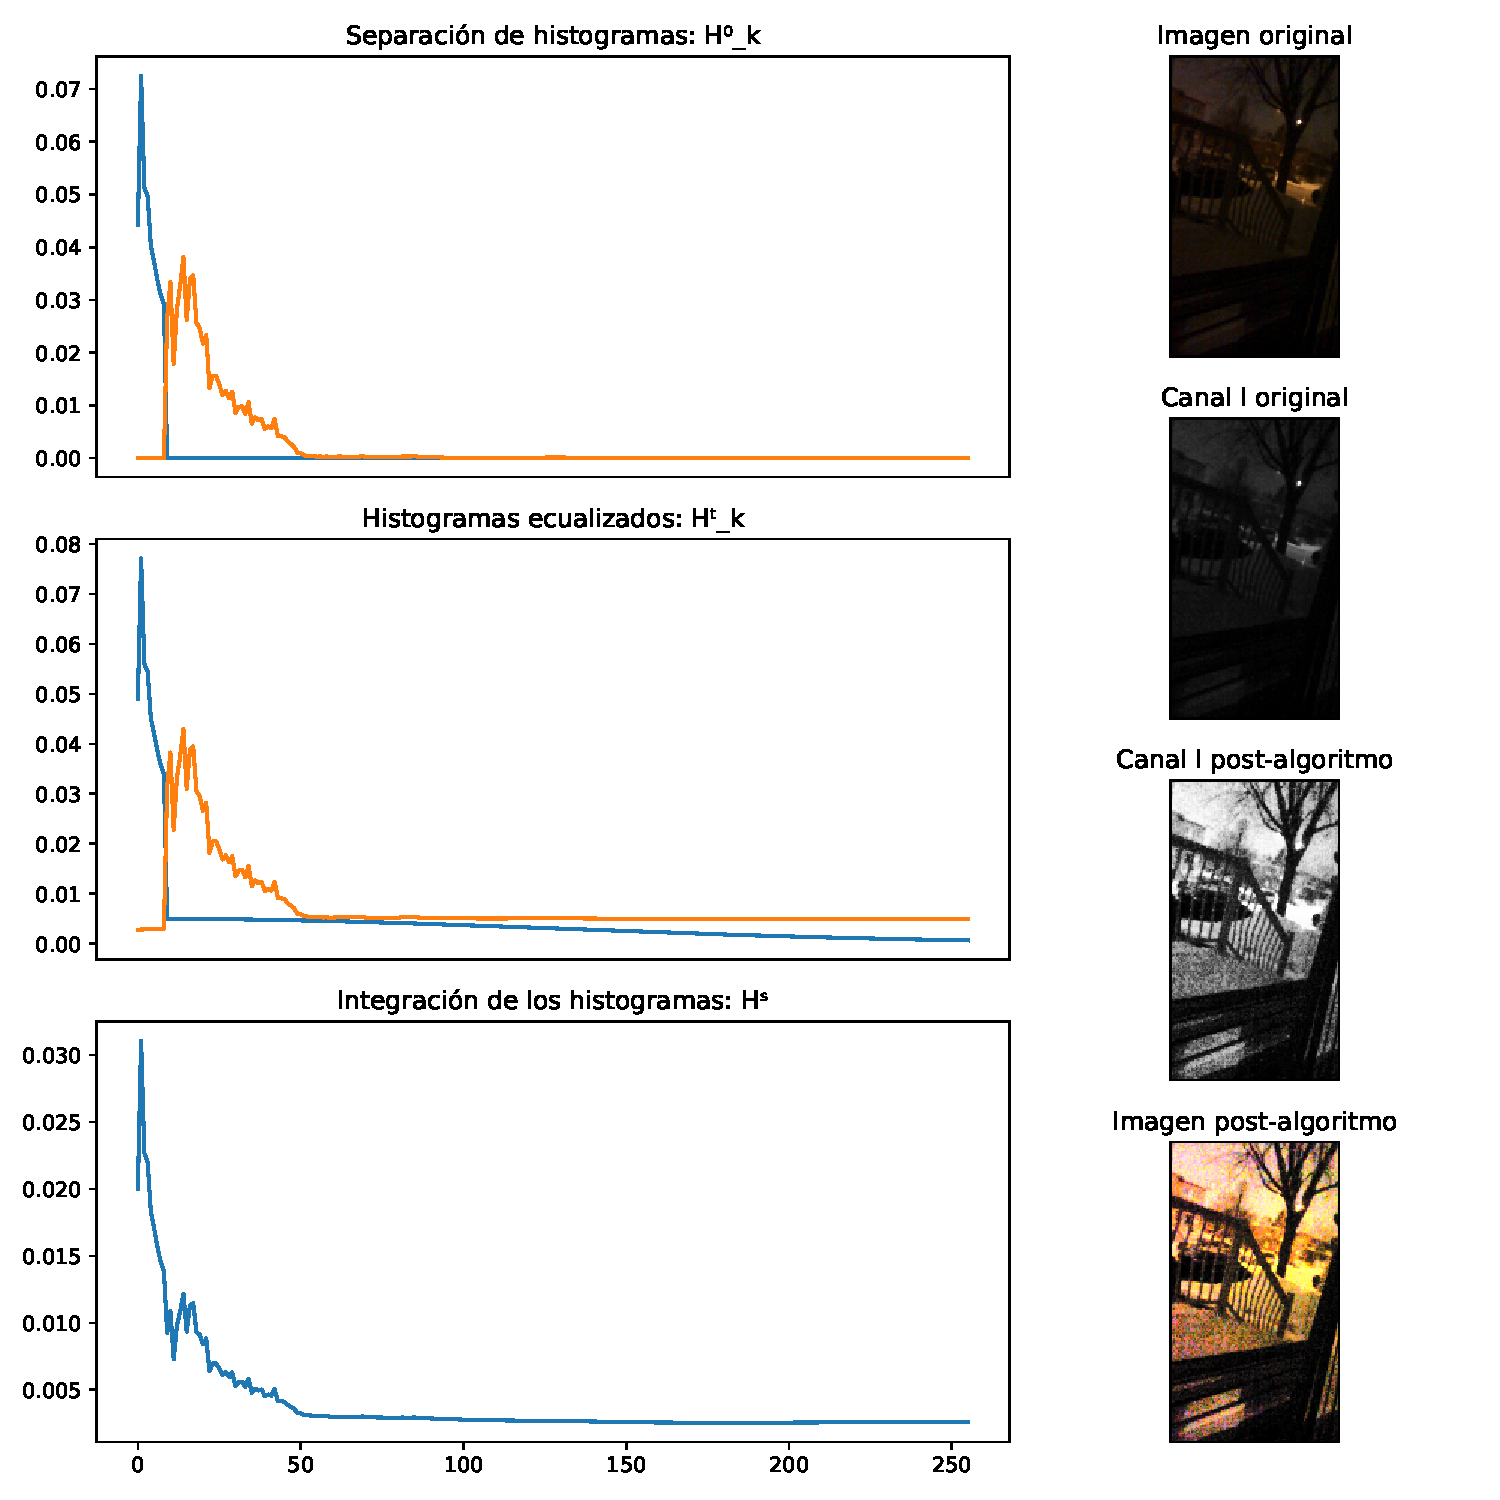
\includegraphics[height=9cm]{imgs/porch-995-005-0.pdf}
  \caption{$\alpha = 0.995, \beta = 0.005, \gamma = 0$}
\end{minipage}
\hfill
\begin{minipage}[c]{0.48\linewidth}
  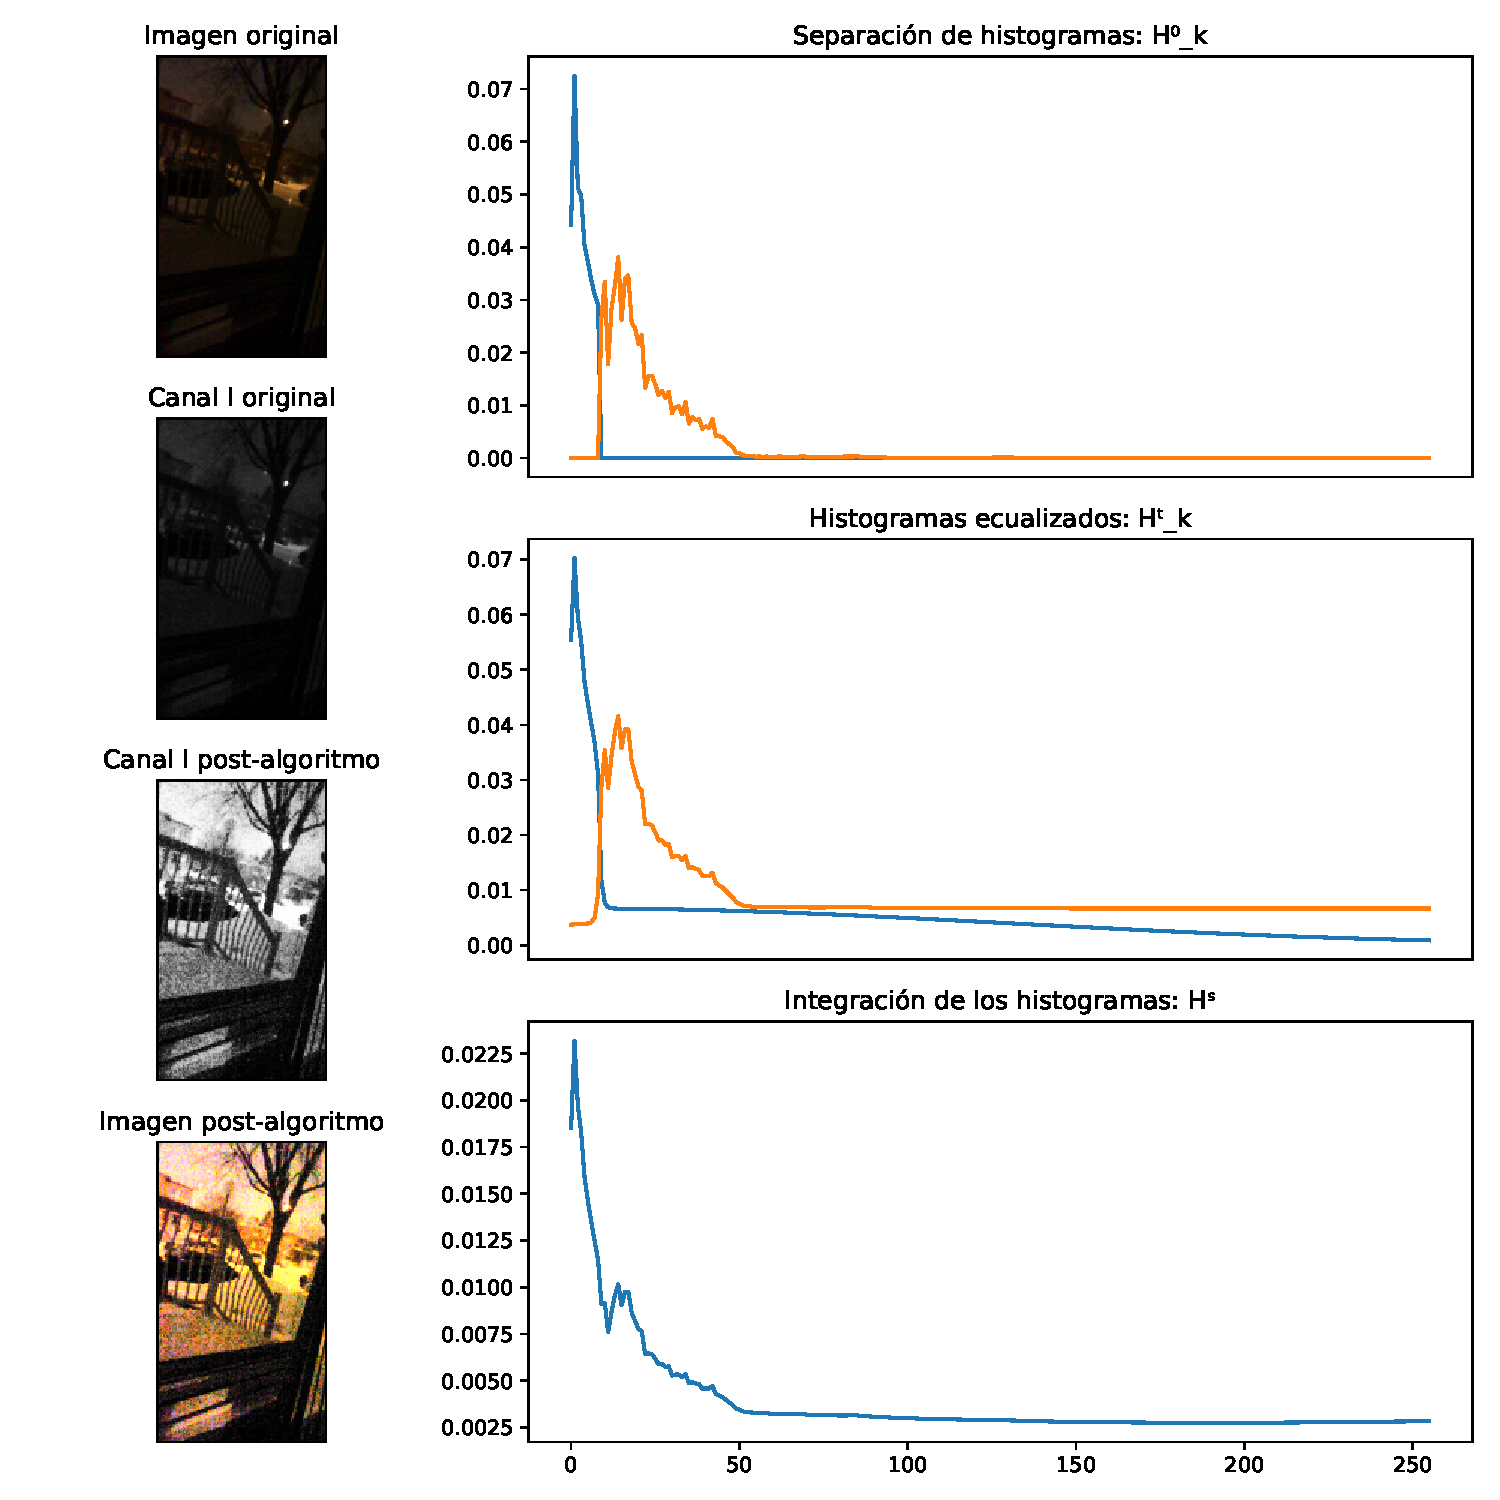
\includegraphics[height=9cm]{imgs/porch-745-005-25.pdf}
  \caption{$\alpha = 0.745, \beta = 0.005, \gamma = 0.25$}
\end{minipage}%
\end{figure}

\begin{figure}[H]
\begin{minipage}[c]{0.48\linewidth}
  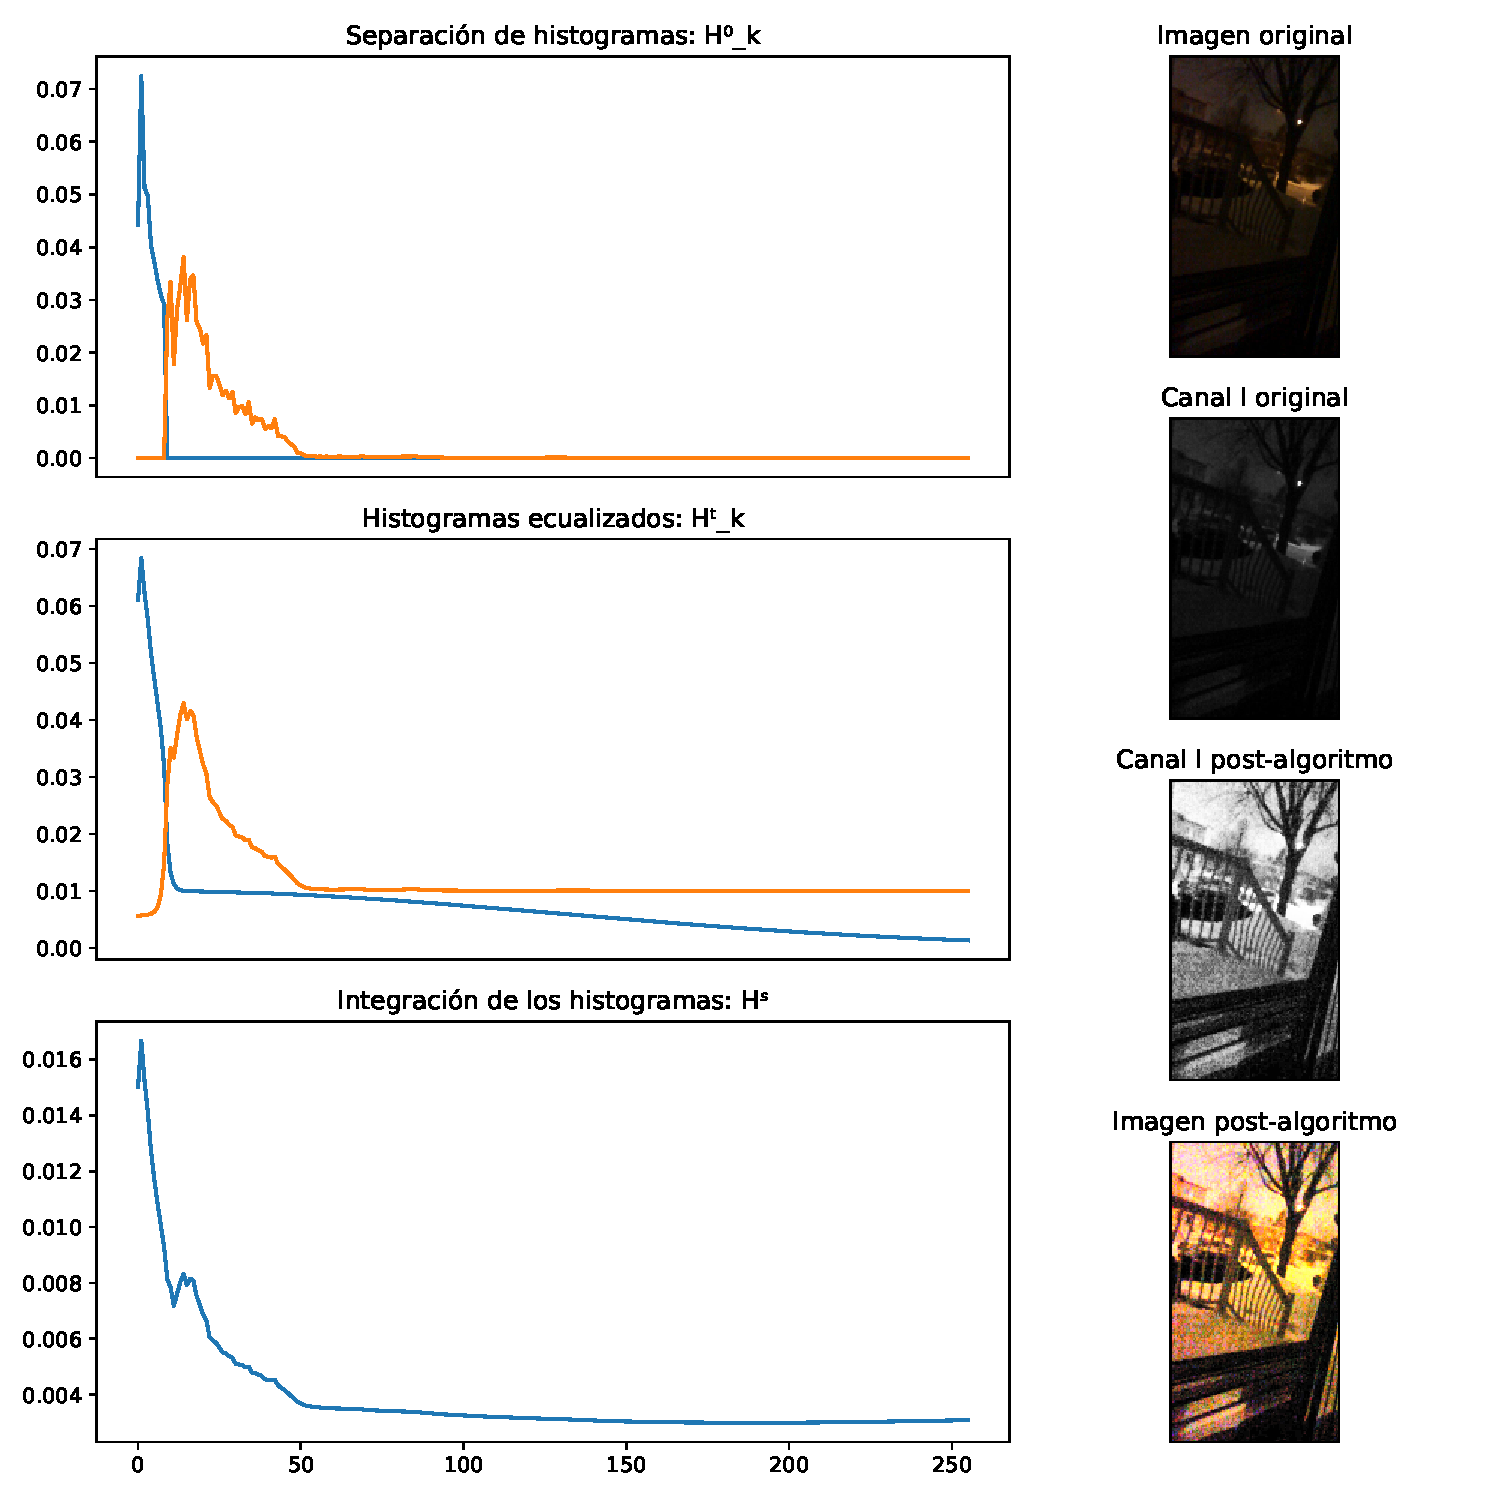
\includegraphics[height=9cm]{imgs/porch-495-005-5.pdf}
  \caption{$\alpha = 0.495, \beta = 0.005, \gamma = 0.5$}
\end{minipage}
\hfill
\begin{minipage}[c]{0.48\linewidth}
  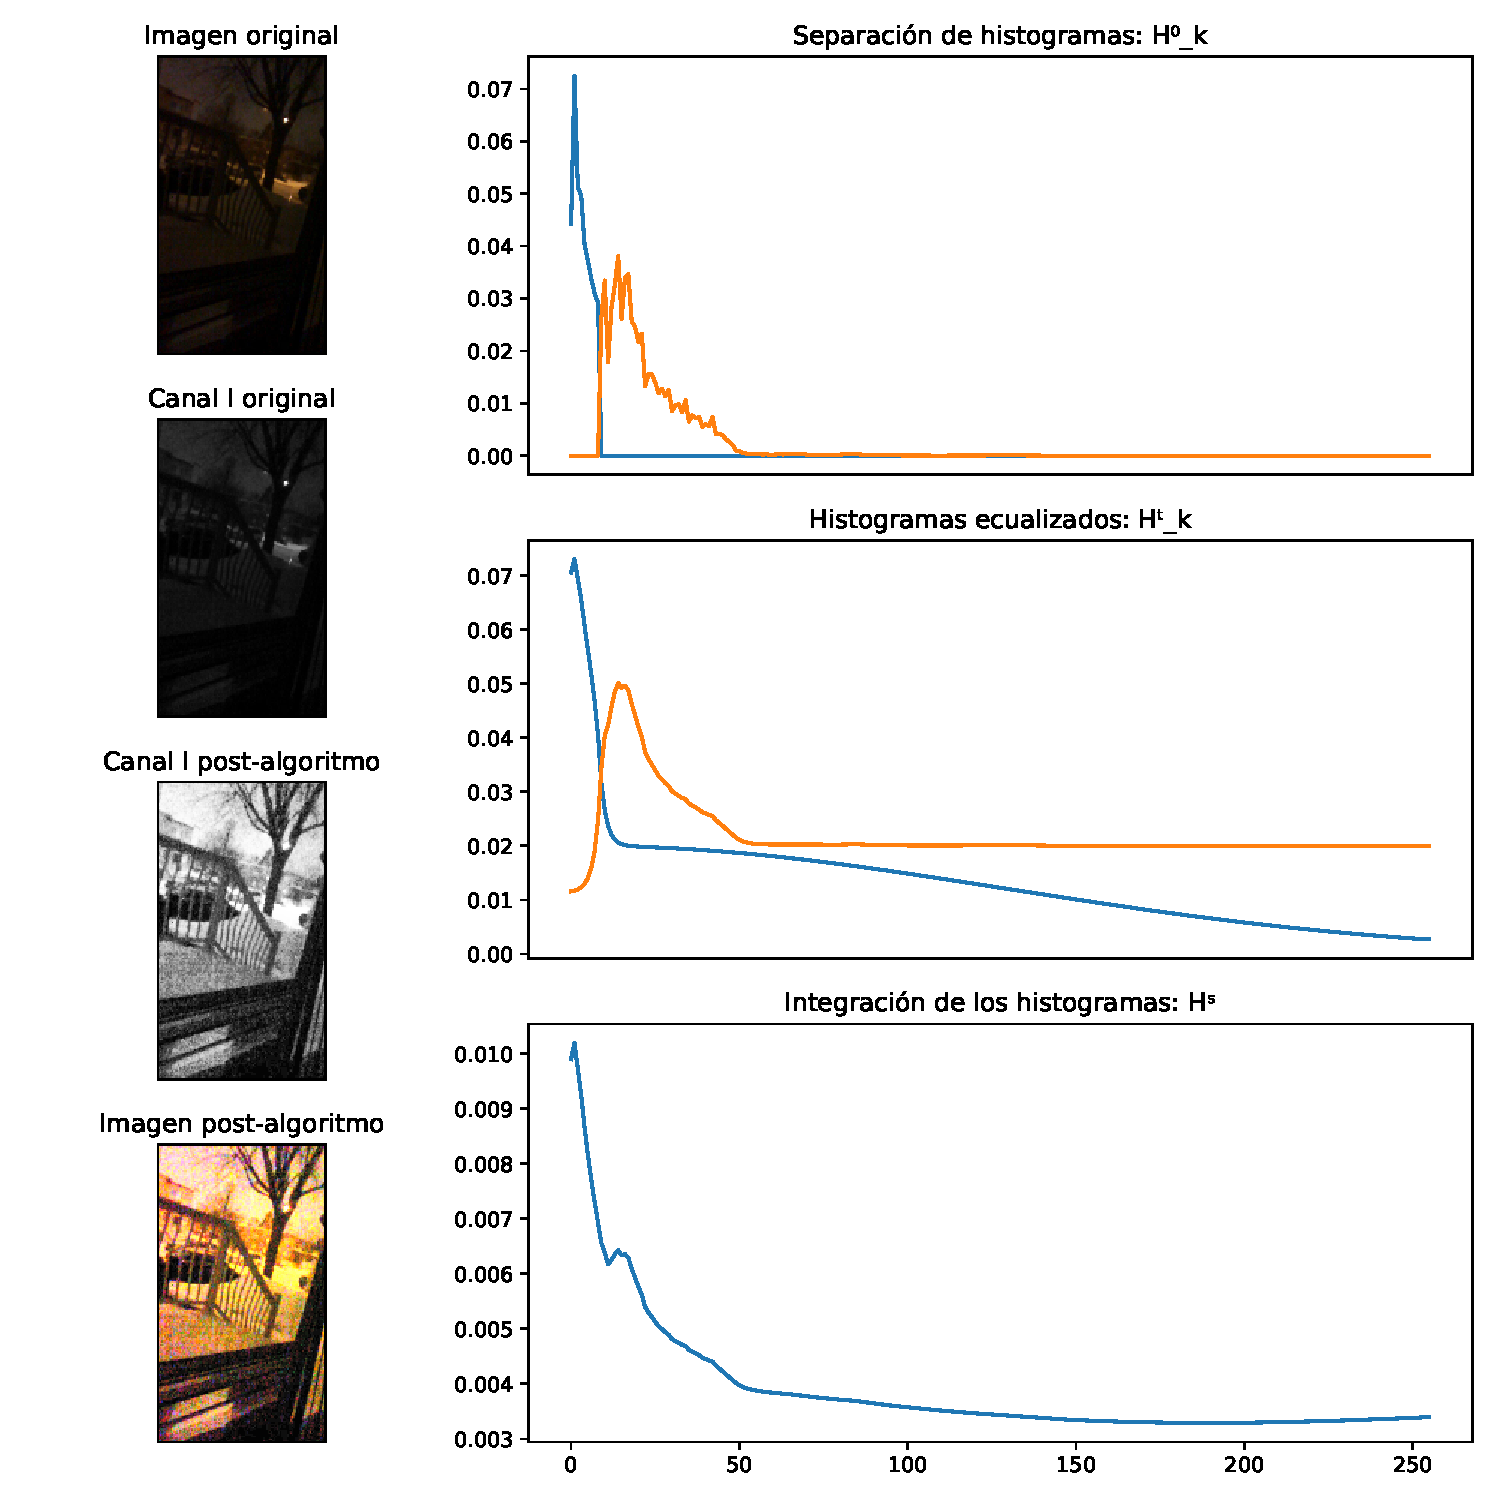
\includegraphics[height=9cm]{imgs/porch-245-005-75.pdf}
  \caption{$\alpha = 0.245, \beta = 0.005, \gamma = 0.75$}
\end{minipage}%
\end{figure}

\begin{figure}[H]
\begin{minipage}[c]{0.48\linewidth}
  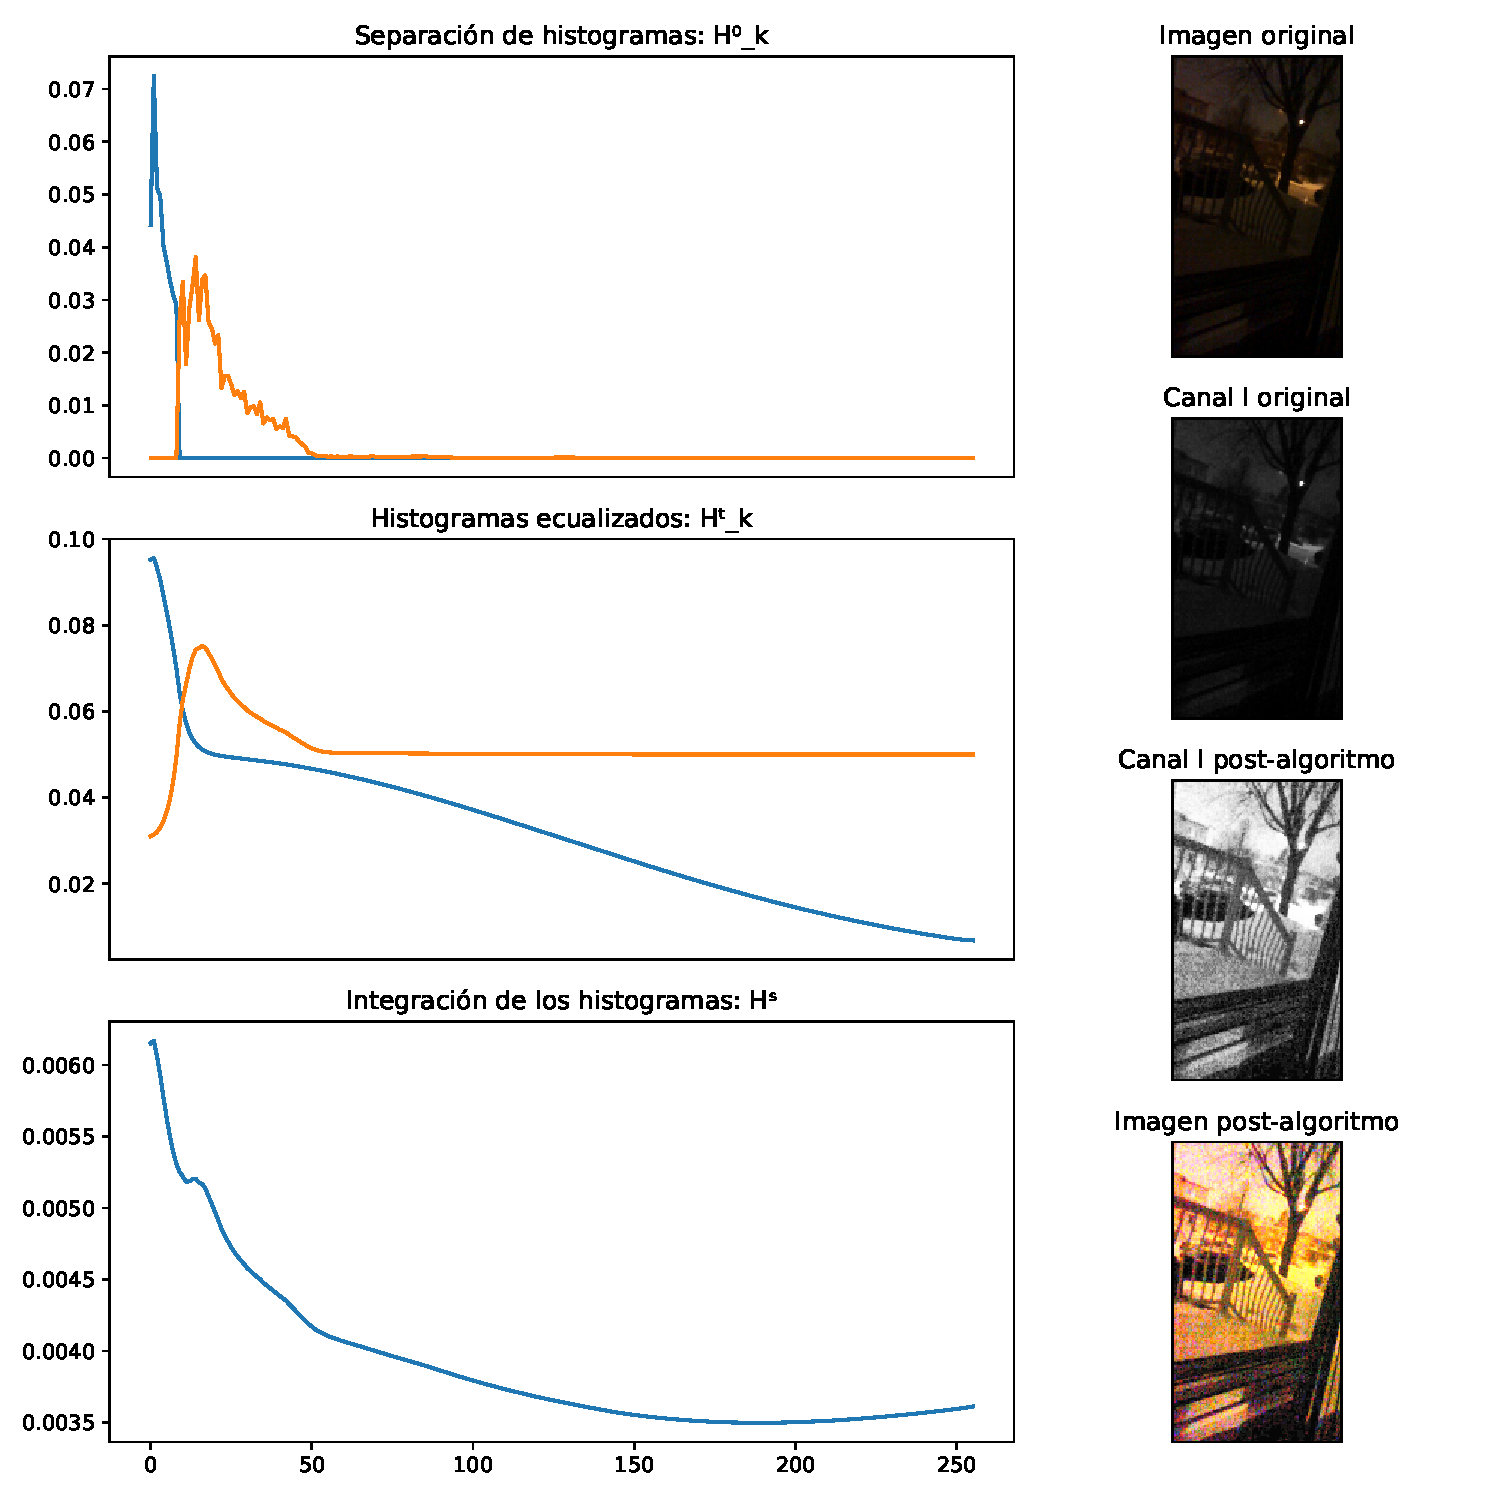
\includegraphics[height=9cm]{imgs/porch-095-005-9.pdf}
  \caption{$\alpha = 0.095, \beta = 0.005, \gamma = 0.9$}
\end{minipage}
\hfill
\begin{minipage}[c]{0.48\linewidth}
  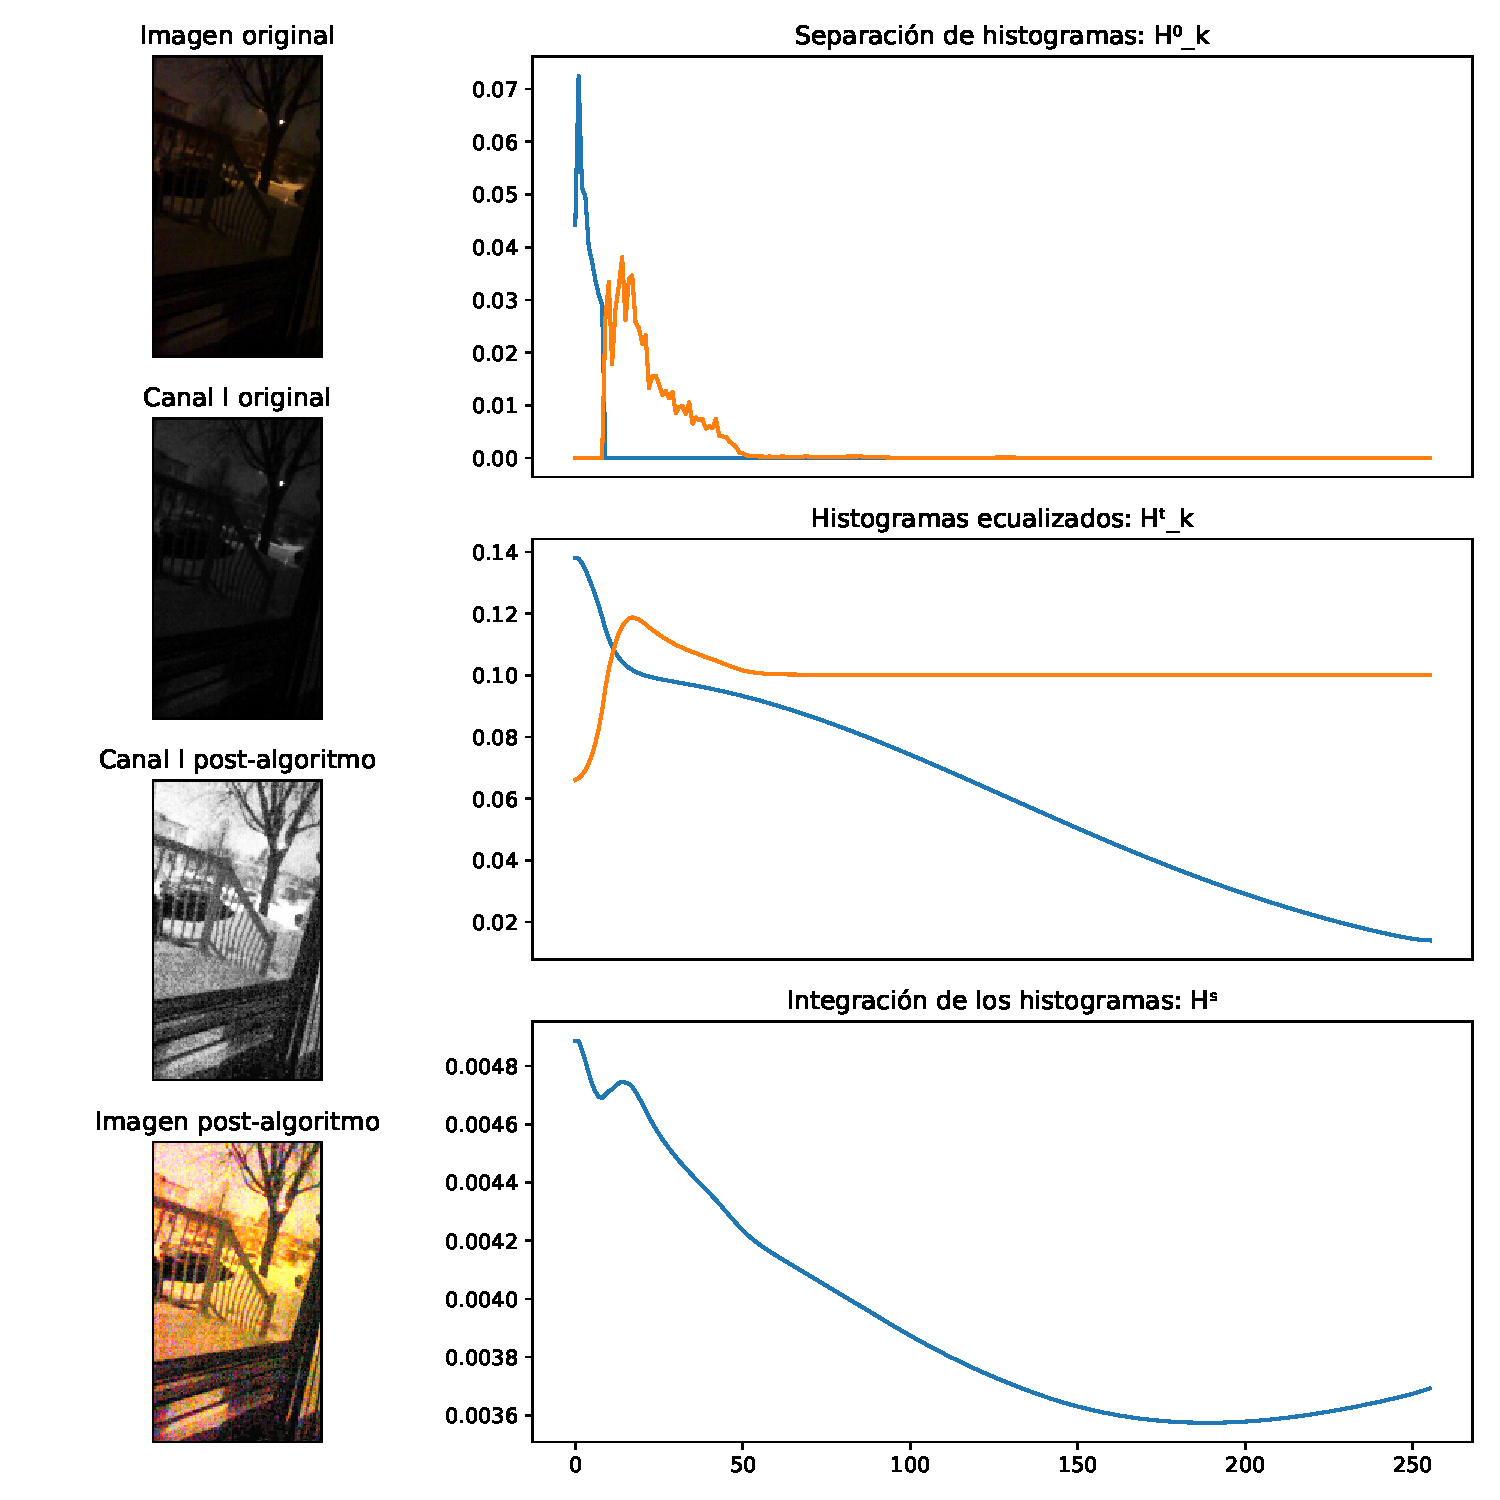
\includegraphics[height=9cm]{imgs/porch-045-005-95.pdf}
  \caption{$\alpha = 0.045, \beta = 0.005, \gamma = 0.95$}
\end{minipage}%
\end{figure}

